\documentclass[12pt]{article}
\usepackage[affil-it]{authblk}
%
\usepackage{amsmath,amssymb,amsthm,ascmac}
\usepackage{float}
\usepackage[dvipdfmx]{graphicx}
\usepackage{subcaption}
\usepackage{here}
\usepackage{pifont}
\usepackage{comment}
\usepackage{tikz}
\usepackage{geometry}
\usepackage{pgfplots}
\usepackage{dsfont}
\usetikzlibrary{patterns}

% \usepackage{natbib}

\usepackage{newtxmath, newtxtext}
\usepackage[scaled=0.90]{helvet} % ss
\usepackage{courier} % tt
\normalfont
\usepackage[T1]{fontenc}

\geometry{left=1.0in,right=1.0in,top=1.0in,bottom=1.0in}
%¥usepackage[top=25truemm,bottom=25truemm,left=10truemm,right=10truemm]{geometry}
\usepackage{setspace}
\setstretch{1.5} %行間の広さ指定

\theoremstyle{definition}
\newtheorem{theorem}{Theorem}
\newtheorem*{theorem*}{Theorem}
\newtheorem{lemma}{Lemma}
\newtheorem*{lemma*}{Lemma}
\newtheorem{proposition}{Proposition}
\newtheorem*{proposition*}{Proposition}
\newtheorem{definition}{Definition}
\newtheorem*{definition*}{Definition}
\newtheorem{corollary}{Corollary}
\newtheorem*{corollary*}{Corollary}
\newtheorem{assumption}{Assumption}
\newtheorem*{assumption*}{Assumption}
\newtheorem{example}{Example}
\newtheorem*{example*}{Example}
\newtheorem*{remark}{Remark}
\newtheorem{algorithm}{Algorithm}
\newtheorem*{algorithm*}{Algorithm}

\newcommand{\bm}[1]{\boldsymbol{#1}}


\begin{document}

\title{Supermodularity and Equilibrium in Games with \\ Peer Effects and Endogenous Network Formation}

\author{Yuya Furusawa}

\date{\today}

\maketitle

\begin{abstract}
Peer effects in the network play an important role in determining individual and aggregate behavior, and many literature argue their importances theoretically and empirically.
However, almost all of the papers treat the network structure as given.
This means that we cannot consider the agents' responses to the economic shocks and alternation of network structure.
We develop the game-theoretic model with endogenous network formation where agents first choose who to connect and then excert efforts.
We show that 1st stage game becomes supermodular game and there exists pure strategy subgame perfect equilibrium.
Then, we give a discussion about multiplicity of equilibrium and comparative statics.
In comparative static analysis, we can show the model incorporates phase transition phenomena.
Finally, we provide a policy implication: key player policy and key link policy.
With considering the endogeneity of the network, we can see the key player and key link might be different with the ones analyzed in the existing literature.
\end{abstract}


\section{Introduction}

% Network with peer effects
Network structures and local interactions play an important role in detemining individual and aggregate behavior.
Individual behavior generates a positive or negative externalities and affects neighbors' behavior, which is referred to as peer effect.
By considering network structure, we can explain the direct effects and indirect effects, that is, the effects of agent's behavior on agents directly connect and indirectly connect.
Recently, many literatures in the economics theoretically and emprically point out this significance.
In these works, it is shown that peer effects are important in many kinds of network, for example, social network, criminal network, firm-to-firm networks where firms invest R\&D activities, networks for labor market participation, educational network, and so on.
In criminal network, when the neighbors are highly devoted to criminal activities such as drug abuses, the agent are more likely to concentrate on the drug usage due to the information or traffickinf from his neighbors.

% Importance of network formation
However, many existing literatures about the networks in economics ignore the mechanism of the network formation.
With fixed networks, some papers\footnote{For production networks, Acemoglu, Carvalho, Ozdaglar, and Tahbaz‐Salehi(2012)~\cite{origin} or Carvalho, Nirei, Saito, and Tahbaz-Salehi(2016)~\cite{nirei}. For a network of military alliances, K\"{o}nig, Rohner, Thoenig, and Zilibotti(2017)~\cite{conflict}} consider the effect of economic shocks or policy changing on the aggregate behavior of the network.
When the economic agents are faced with the alteration of the environment where they are, they respond to them in order to mitigate the shocks.
Finally, the network structure will be changed.
Therefore, it is significant to consider the mechanism of network formation to analyze the impact of policy intervaton.
In this paper, we propose the way to overcome this problem by incorporating the endogenous network formation to the model.

% Summary of model
We develop the two stage dynamic game, where agents form links to other agents in the first stage and agents excert efforts in the second stage.
Second stage game is eccensially same with the model in Ballester, Calv\'{o}-Armengol, and Zenou(2006)~\cite{whowho}.
Agents simultaneously choose a nonnegative effort level and the agents' payoffs depend on not only their own effort but also neighbors' effort.
The agents' efforts generates the positive externalities, so called "peer effects", to the connected agents in the network.
We extend the model of Ballester, Calvo-Armengol, and Zenou(2006)~\cite{whowho} to the endogenous network by introducing first stage game, choosing neighbors.
In the first stage, agents simultaneously choose their neighbors from the neighbors in the potential network, which represents the maximual possible conncetion without any limitations.
When agents decide who to connect, they incur the link-specific costs, which is a key factor for determining the network.
The link formation costs (and benefits of efforts) make the heterogeneity across the agents, which leads to the various types of networks.
The interpretion of links, effort, and link formation cost depend on the application we consider.
For example, when we consider the criminal network, links, effort, and formation cost represent the flow of criminal informtion or trafficking weapons, the intension of criminal acrivity, and the geographical distance or the probability of capture, respectively.
When we apply to the R\&D network, we can think of links as the contract to colaboration, effort as the investment to R\&D, and link formation cost as the negotiation cost or financial cost to sign a constract.
We consider the subgame perfect equilibrium where all agents take pure starategies in the both stages.

% Interpretation
We can interpret the model in some different ways.
First, we can think of this model as the web advertisement network.
Node, link, link formation cost, and effort represent web sites, advertisement on other sites, fee, and investment on the web contents respectively.
If connected sites invest on the site and the number of viewers increase, more viewers visit the site and there exists a incentive to invest more.
In another interpretation, we can regard this model as the drug trafficking network.
Municipalities, drug trafficking, and the amount of drug used are represented by nodes, links and efforts respectively.
Link formation cost means the probability of capture during trafficking.
In Dell(2015)~\cite{Dell}, drug are trafficked across municiparities in Mexico, and exported to U.S.
Probabilty of capture, which is represented by  link formation cost, depends on the policy of the city and government.
Moreover, Dell(2015)~\cite{Dell} indicates that there exists spillover effects when the policy maker leads one location to become less active to illicit activities, and this coincides with our model where peer effects in effort levels and choosing neighbor strategy exist.

% Summary of results
We establish that pure strategy subgame perfect equilibrium always exists.
Due to the result in Ballester, Calv\'{o}-Armengol, and Zenou(2006)~\cite{whowho}, second stage Nash equilibrium always exists and it is unique.
Given this equilibrium, by backward induction, we show first stage becomes supermodular game.
Then, by well known properties of supermodurarity, we can see the first stage equilibrium always exists, and we have the greatest and smallest ones, so equilibrium may not be unique.
We focus on the greatest equilibrium which can be obtained by some best response dynamics algorithm.
In comparative static analysis in link formation costs, we see that reduction in the costs leads to larger network because agents are more likely to connect to other agents.
Realized network is discontinuous in the link formation costs, so changes in the costs leads to discontinuous changes in the network.
We give a example that tiny change in the link formation costs leads to drastic change of the network structure, "phase transition".
We analyze a key player policy in endogenous networks as in the previous literature.
Key player is the agent in the potential network who makes largest reduction of aggregate effort level once he removed from the potential network.
However, it is difficult to find key players from the link formation costs because its discontinuity.
We give a example that key player in the endogenous network and in the exogenous (key player defined in the previous literatures) might be different.
This example shows that witout considering the mechanism of the network formation, we might have a wrong policy implication.
Similarly, we analyze key link policy which is introduced in this paper for the first time, and we see we may have wrong policy without considering the endogenous network formation.

% Literature Review
This paper contributes to the growing literatures on the endogenous networks.
Endogeneity of the network is one of the hottest topics in the field of econimic networks and many researchers tackle this problem.
Oberfield(2018)~\cite{ober}, and Acemoglu and Azar(2019)~\cite{endo_net} argue the endogenous production networks.
In their model, the productivity of the firms is determined by the input or supplier, and the its customer, who use its output as input, and final consumers generates the firms' profit.
This productivity is the key factor for network formation, and, in equilibrium, input-output architecture endogenously emerge.
Farboodi(2014)~\cite{farboodi} and other papers\footnote{For examples, Cohen-Cole, Patacchini, and Zenou(2010)~\cite{cohen}, Acemoglu, Ozdaglar, and Tahbaz-Salehi(2015)~\cite{acemo2015} and Babus(2016)~\cite{babus}} argue the endogenous formation of financial networks.
Recently, many papers theoretically and empirically work for other networks\footnote{Canen, Jackson, and Trebbi(2019)~\cite{canen}, Marco, Eleonora, and Edoardo(2019)~\cite{Marco2019}, Margherita, and Mariapia(2015)~\cite{marg}, Tintelnot, Kikkawa, Mogstad, and Dhyne(2018)~\cite{Tin}}.
Our model is one of the models in network game, such as Jackson, and Wolinsky(1996), Galeotti, Goyal, Jackson, Vega-Redondo, and Yariv(2010)~\cite{galeo} and Bramoull\'{e}, Kranton, and D'Amours(2014).

This paper also related to the peer effect in the networks.
The importance of peer effect is often pointed out originally in Rees(1966)~\cite{Rees} or recently Banerjee, Chandrasekhar, Duflo, and Jackson(2013)~\cite{ban}.
Many papers develop the analysis of peer effects in the network.
Calv\'{o}-Armengol, Patacchini, and Zenou(2009)~\cite{edu} theoretically and empirically analyzes the peer effect for the educational achivement.
Liu, Patacchini, Zenou, and Lee(2012)~\cite{criminal} and Dell(2015)~\cite{Dell} argue the positive externalities in the criminal network.
Bramoull\'{e}, Djebbari, and Fortin(2009)~\cite{identificationpeer} and Liu, Patacchini, and Zenou(2014)~\cite{endopeer} propose the conditions we can identify the peer effect in the network and analyze social network empirically.
K\"{o}nig, Liu, and Zenou(2019)~\cite {RandD} provide theoretical and empirical discussion about R\&D network where peer effects exist.
This paper also considers the peer effect in the network.
As discusses below, due to this positive externality, we can theoretically extend these models to the endogenous network formation.

% Closely Related Literature
This paper is closely related to Kim, Patacchini, Picard, and Zenou(2017)~\cite{Urban} which considers the social relationship formation in the urban geographical space.
They consider the model where a contiuum of agents distributes over the line segment and decides the intensity of interactions to the agents who lives in the other point of the segment.
The agents' payoff and the positive externalities of the interactions are eccentially same with our model and Ballester, Calv\'{o}-Armengol, and Zenou(2006)~\cite{whowho} (and other literatures).
Although the number of agents is infinite, we can treat their model as the network formation model.\footnote{In empirical part, they discritize the agents and consider the adjacency matrix as our model.}
The key factor of network formation in their paper is the distribution of agents and the cost of interations which is measured by geographic distance.
There are two differences in this paper and ours.
First, in their model, the cost of interactions is only determined by the distance of two agents.
In many cases, interactions are affected by various kinds of obstacles, such as psychological barrier and financial cost.
In contrast, our model can incorporate any kinds of interaction costs, and it enables us to consider any kinds of economic situations in our framework.
Second, they consider the weighted relationships and agents decide the intensity of interaction to every other agents.
Due to this feature, we can remove the any kinds of discontinuity and compute the network structure and the weights of links analytically.
However, analytical solution always shows that equilibrium network is always complete network, that is every agent connects all other agents in the network.
Our model can explain the formation of any structure of the networks.

Hiller(2017)~\cite{hiller} is also related to our paper.
He develops the very similar model with ours: agents choose their neighbors and decide the level of efforts.
He considers the general payoff function which include the payoff function in our model.
But he considers the static game where all agents choose neighbors and effort levels simultaneously.
In addition, the costs of link formation is determined by the number of links.
This construction of the model lacks the uniqueness of the equilibrium, Nash equilibrium.
Our model can have a kind of uniqueness of the equilibrium by setting the game dynamic.

The rest of the paper is organized as follows.
Section 2 describes the model.
In section 3, we first give the definition of the equilibrium and present the result on its existence and uniqueness.
We also present the result on comparative statics in this section.
In section 4, we comment on the key player and Section 5 concludes.
All proofs used to show the reults in this paper are attached in the Appendix(Section 6).


\section{Model}

There are $n$ agents in the economy, and denote the set of agents $N = \{ 1, \cdots, n\}$.
We assume $n$ is finite and $n \ge 2$.

The game consists of two-stage game: {\it{choosing neighbors}} and {\it{choosing an effort level}}.
Initially, agents are connected in the potential network $g^p$.
We consider the network $g^p$ is connected, directed and unweighted.
The potential network $g^p$ is represented by adjacency matrix $\bm{G}^p = {(g_{ij}^p)}_{ij}$ where, for any $i \neq j$,
\[ g_{ij}^p =
	\begin{cases}
		1 \  (\text{if $i$ has a link to $j$ in $g^p $}) \\
		0 \  (\text{otherwise})
	\end{cases} \]
Note that $\bm{G}^p$ can be asymetric and $g_{ii}^p = 0$ for all $i$.
Denote the set of agent $i$'s neighbors in the potential network $N_i(g^p) = \{ j \in N | g_{ij}^p = 1 \}$.
In the first stage, each agent $i$ simultaneously chooses the partners from the potential neighbors $N_i(g^p)$.
This strategy can be represented by $\psi_i = (\psi_{i1}, \cdots, \psi_{in})$ such that $\psi_{ij} \in \{0, 1\}$ for all $j \in N$, $\psi_{ii}=0$ for all $i \in N$, and $\psi_{ij} = 0$ for all $j \notin N_i(g^p)$.
Note that $\psi_i \in \Psi_i = \{0, 1\}^{n}$ and $\Psi = \prod_{i=1}^n \Psi_i$.
We assume that when forming a link, each agent incurs a cost $c_{ij} \ge 0$, and denote its matrix $\bm{C} = {(c_{ij})}_{ij}$.\footnote{We assume that $c_{ij} = 0$ for $ij$ such that $g_{ij}^p = 0$.}
The link formation cost represents, for example, geographic distance or psychological barrier.
Since $\psi_i$ depends on potential network $g^p$ and costs $\bm{C}$, to emphasize it, we denote $\psi_i(g^p, \bm{C})$.
We denote its profile $\bm{\psi}(g^p, \bm{C}) = \prod_{i=1}^n \psi_i(g^p, \bm{C})$.
After forming links, the network $g$ is realized.
Figure \ref{fig:dif} represents the difference between potential network and realized network.
Only links which exist in the potential network can be realized.

%% Figure of the difference between potential network and realized network
\begin{figure}[h]
\centering
\tikzset{every picture/.style={line width=0.75pt}}        
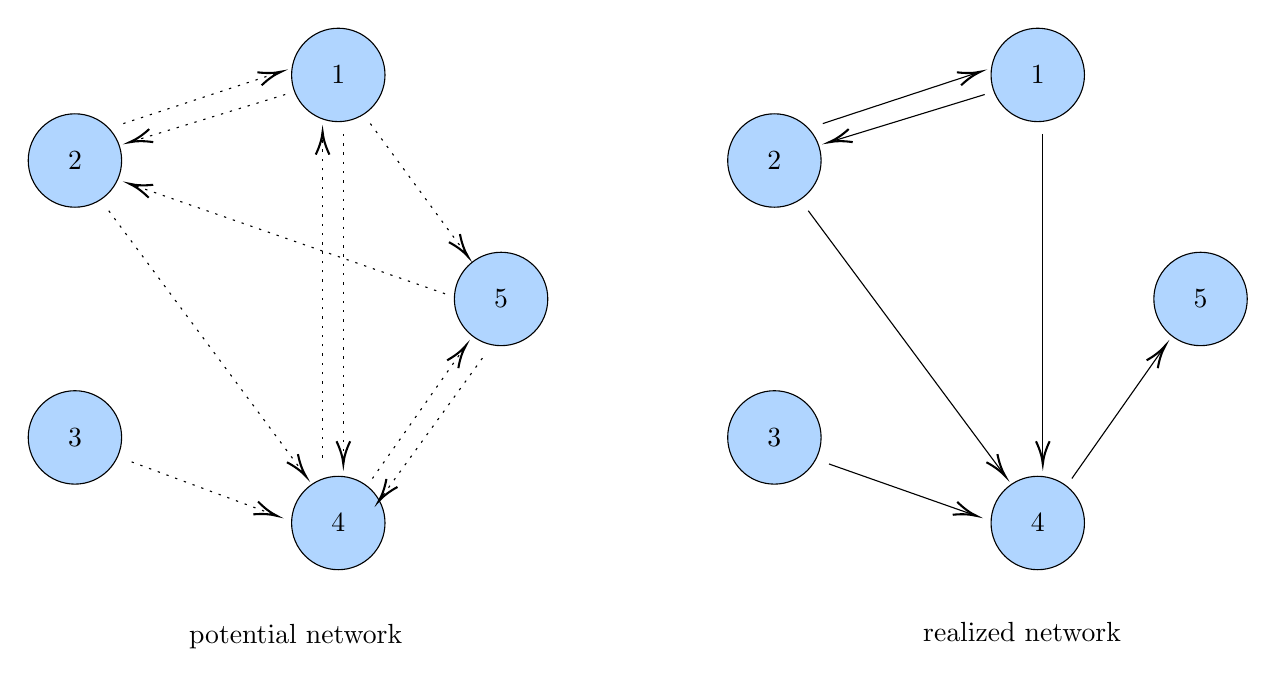
\begin{tikzpicture}[x=0.75pt,y=0.75pt,yscale=-1,xscale=1]
\draw  [fill={rgb, 255:red, 103; green, 174; blue, 255 }  ,fill opacity=0.52 ] (201.07,65.56) .. controls (201.07,53.13) and (211.15,43.06) .. (223.57,43.06) .. controls (236,43.06) and (246.07,53.13) .. (246.07,65.56) .. controls (246.07,77.98) and (236,88.06) .. (223.57,88.06) .. controls (211.15,88.06) and (201.07,77.98) .. (201.07,65.56) -- cycle ;
\draw  [fill={rgb, 255:red, 103; green, 174; blue, 255 }  ,fill opacity=0.52 ] (74.18,106.79) .. controls (74.18,94.36) and (84.25,84.29) .. (96.68,84.29) .. controls (109.1,84.29) and (119.18,94.36) .. (119.18,106.79) .. controls (119.18,119.21) and (109.1,129.29) .. (96.68,129.29) .. controls (84.25,129.29) and (74.18,119.21) .. (74.18,106.79) -- cycle ;
\draw  [fill={rgb, 255:red, 103; green, 174; blue, 255 }  ,fill opacity=0.52 ] (279.5,173.5) .. controls (279.5,161.07) and (289.57,151) .. (302,151) .. controls (314.43,151) and (324.5,161.07) .. (324.5,173.5) .. controls (324.5,185.93) and (314.43,196) .. (302,196) .. controls (289.57,196) and (279.5,185.93) .. (279.5,173.5) -- cycle ;
\draw  [fill={rgb, 255:red, 103; green, 174; blue, 255 }  ,fill opacity=0.52 ] (74.18,240.21) .. controls (74.18,227.79) and (84.25,217.71) .. (96.68,217.71) .. controls (109.1,217.71) and (119.18,227.79) .. (119.18,240.21) .. controls (119.18,252.64) and (109.1,262.71) .. (96.68,262.71) .. controls (84.25,262.71) and (74.18,252.64) .. (74.18,240.21) -- cycle ;
\draw  [fill={rgb, 255:red, 103; green, 174; blue, 255 }  ,fill opacity=0.52 ] (201.07,281.44) .. controls (201.07,269.02) and (211.15,258.94) .. (223.57,258.94) .. controls (236,258.94) and (246.07,269.02) .. (246.07,281.44) .. controls (246.07,293.87) and (236,303.94) .. (223.57,303.94) .. controls (211.15,303.94) and (201.07,293.87) .. (201.07,281.44) -- cycle ;
\draw  [dash pattern={on 0.84pt off 2.51pt}]  (239,89) -- (284.82,151.39) ;
\draw [shift={(286,153)}, rotate = 233.71] [color={rgb, 255:red, 0; green, 0; blue, 0 }  ][line width=0.75]    (10.93,-3.29) .. controls (6.95,-1.4) and (3.31,-0.3) .. (0,0) .. controls (3.31,0.3) and (6.95,1.4) .. (10.93,3.29)   ;
\draw  [dash pattern={on 0.84pt off 2.51pt}]  (198,75) -- (124.91,97.41) ;
\draw [shift={(123,98)}, rotate = 342.95] [color={rgb, 255:red, 0; green, 0; blue, 0 }  ][line width=0.75]    (10.93,-3.29) .. controls (6.95,-1.4) and (3.31,-0.3) .. (0,0) .. controls (3.31,0.3) and (6.95,1.4) .. (10.93,3.29)   ;
\draw  [dash pattern={on 0.84pt off 2.51pt}]  (226,94) -- (226,251) ;
\draw [shift={(226,253)}, rotate = 270] [color={rgb, 255:red, 0; green, 0; blue, 0 }  ][line width=0.75]    (10.93,-3.29) .. controls (6.95,-1.4) and (3.31,-0.3) .. (0,0) .. controls (3.31,0.3) and (6.95,1.4) .. (10.93,3.29)   ;
\draw  [dash pattern={on 0.84pt off 2.51pt}]  (120,89) -- (194.1,64.62) ;
\draw [shift={(196,64)}, rotate = 521.79] [color={rgb, 255:red, 0; green, 0; blue, 0 }  ][line width=0.75]    (10.93,-3.29) .. controls (6.95,-1.4) and (3.31,-0.3) .. (0,0) .. controls (3.31,0.3) and (6.95,1.4) .. (10.93,3.29)   ;
\draw  [dash pattern={on 0.84pt off 2.51pt}]  (113,131) -- (206.81,257.39) ;
\draw [shift={(208,259)}, rotate = 233.42000000000002] [color={rgb, 255:red, 0; green, 0; blue, 0 }  ][line width=0.75]    (10.93,-3.29) .. controls (6.95,-1.4) and (3.31,-0.3) .. (0,0) .. controls (3.31,0.3) and (6.95,1.4) .. (10.93,3.29)   ;
\draw  [dash pattern={on 0.84pt off 2.51pt}]  (124,252) -- (192.13,277.3) ;
\draw [shift={(194,278)}, rotate = 200.38] [color={rgb, 255:red, 0; green, 0; blue, 0 }  ][line width=0.75]    (10.93,-3.29) .. controls (6.95,-1.4) and (3.31,-0.3) .. (0,0) .. controls (3.31,0.3) and (6.95,1.4) .. (10.93,3.29)   ;
\draw  [dash pattern={on 0.84pt off 2.51pt}]  (216,250) -- (216,95) ;
\draw [shift={(216,93)}, rotate = 450] [color={rgb, 255:red, 0; green, 0; blue, 0 }  ][line width=0.75]    (10.93,-3.29) .. controls (6.95,-1.4) and (3.31,-0.3) .. (0,0) .. controls (3.31,0.3) and (6.95,1.4) .. (10.93,3.29)   ;
\draw  [dash pattern={on 0.84pt off 2.51pt}]  (240,260) -- (283.85,197.64) ;
\draw [shift={(285,196)}, rotate = 485.11] [color={rgb, 255:red, 0; green, 0; blue, 0 }  ][line width=0.75]    (10.93,-3.29) .. controls (6.95,-1.4) and (3.31,-0.3) .. (0,0) .. controls (3.31,0.3) and (6.95,1.4) .. (10.93,3.29)   ;
\draw  [dash pattern={on 0.84pt off 2.51pt}]  (293,202) -- (244.17,269.38) ;
\draw [shift={(243,271)}, rotate = 305.93] [color={rgb, 255:red, 0; green, 0; blue, 0 }  ][line width=0.75]    (10.93,-3.29) .. controls (6.95,-1.4) and (3.31,-0.3) .. (0,0) .. controls (3.31,0.3) and (6.95,1.4) .. (10.93,3.29)   ;
\draw  [dash pattern={on 0.84pt off 2.51pt}]  (275,171) -- (124.89,118.66) ;
\draw [shift={(123,118)}, rotate = 379.22] [color={rgb, 255:red, 0; green, 0; blue, 0 }  ][line width=0.75]    (10.93,-3.29) .. controls (6.95,-1.4) and (3.31,-0.3) .. (0,0) .. controls (3.31,0.3) and (6.95,1.4) .. (10.93,3.29)   ;
\draw  [fill={rgb, 255:red, 103; green, 174; blue, 255 }  ,fill opacity=0.52 ] (538.07,65.56) .. controls (538.07,53.13) and (548.15,43.06) .. (560.57,43.06) .. controls (573,43.06) and (583.07,53.13) .. (583.07,65.56) .. controls (583.07,77.98) and (573,88.06) .. (560.57,88.06) .. controls (548.15,88.06) and (538.07,77.98) .. (538.07,65.56) -- cycle ;
\draw  [fill={rgb, 255:red, 103; green, 174; blue, 255 }  ,fill opacity=0.52 ] (411.18,106.79) .. controls (411.18,94.36) and (421.25,84.29) .. (433.68,84.29) .. controls (446.1,84.29) and (456.18,94.36) .. (456.18,106.79) .. controls (456.18,119.21) and (446.1,129.29) .. (433.68,129.29) .. controls (421.25,129.29) and (411.18,119.21) .. (411.18,106.79) -- cycle ;
\draw  [fill={rgb, 255:red, 103; green, 174; blue, 255 }  ,fill opacity=0.52 ] (616.5,173.5) .. controls (616.5,161.07) and (626.57,151) .. (639,151) .. controls (651.43,151) and (661.5,161.07) .. (661.5,173.5) .. controls (661.5,185.93) and (651.43,196) .. (639,196) .. controls (626.57,196) and (616.5,185.93) .. (616.5,173.5) -- cycle ;
\draw  [fill={rgb, 255:red, 103; green, 174; blue, 255 }  ,fill opacity=0.52 ] (411.18,240.21) .. controls (411.18,227.79) and (421.25,217.71) .. (433.68,217.71) .. controls (446.1,217.71) and (456.18,227.79) .. (456.18,240.21) .. controls (456.18,252.64) and (446.1,262.71) .. (433.68,262.71) .. controls (421.25,262.71) and (411.18,252.64) .. (411.18,240.21) -- cycle ;
\draw  [fill={rgb, 255:red, 103; green, 174; blue, 255 }  ,fill opacity=0.52 ] (538.07,281.44) .. controls (538.07,269.02) and (548.15,258.94) .. (560.57,258.94) .. controls (573,258.94) and (583.07,269.02) .. (583.07,281.44) .. controls (583.07,293.87) and (573,303.94) .. (560.57,303.94) .. controls (548.15,303.94) and (538.07,293.87) .. (538.07,281.44) -- cycle ;
\draw    (535,75) -- (461.91,97.41) ;
\draw [shift={(460,98)}, rotate = 342.95] [color={rgb, 255:red, 0; green, 0; blue, 0 }  ][line width=0.75]    (10.93,-3.29) .. controls (6.95,-1.4) and (3.31,-0.3) .. (0,0) .. controls (3.31,0.3) and (6.95,1.4) .. (10.93,3.29)   ;
\draw    (563,94) -- (563,251) ;
\draw [shift={(563,253)}, rotate = 270] [color={rgb, 255:red, 0; green, 0; blue, 0 }  ][line width=0.75]    (10.93,-3.29) .. controls (6.95,-1.4) and (3.31,-0.3) .. (0,0) .. controls (3.31,0.3) and (6.95,1.4) .. (10.93,3.29)   ;
\draw    (457,89) -- (531.1,64.62) ;
\draw [shift={(533,64)}, rotate = 521.79] [color={rgb, 255:red, 0; green, 0; blue, 0 }  ][line width=0.75]    (10.93,-3.29) .. controls (6.95,-1.4) and (3.31,-0.3) .. (0,0) .. controls (3.31,0.3) and (6.95,1.4) .. (10.93,3.29)   ;
\draw    (450,131) -- (543.81,257.39) ;
\draw [shift={(545,259)}, rotate = 233.42000000000002] [color={rgb, 255:red, 0; green, 0; blue, 0 }  ][line width=0.75]    (10.93,-3.29) .. controls (6.95,-1.4) and (3.31,-0.3) .. (0,0) .. controls (3.31,0.3) and (6.95,1.4) .. (10.93,3.29)   ;
\draw    (460,253) -- (529.11,277.34) ;
\draw [shift={(531,278)}, rotate = 199.4] [color={rgb, 255:red, 0; green, 0; blue, 0 }  ][line width=0.75]    (10.93,-3.29) .. controls (6.95,-1.4) and (3.31,-0.3) .. (0,0) .. controls (3.31,0.3) and (6.95,1.4) .. (10.93,3.29)   ;
\draw    (577,260) -- (620.85,197.64) ;
\draw [shift={(622,196)}, rotate = 485.11] [color={rgb, 255:red, 0; green, 0; blue, 0 }  ][line width=0.75]    (10.93,-3.29) .. controls (6.95,-1.4) and (3.31,-0.3) .. (0,0) .. controls (3.31,0.3) and (6.95,1.4) .. (10.93,3.29)   ;
\draw (223.57,65.56) node   {$1$};
\draw (96.68,106.79) node   {$2$};
\draw (96.68,240.21) node   {$3$};
\draw (223.57,281.44) node   {$4$};
\draw (302,173.5) node   {$5$};
\draw (560.57,65.56) node   {$1$};
\draw (433.68,106.79) node   {$2$};
\draw (433.68,240.21) node   {$3$};
\draw (560.57,281.44) node   {$4$};
\draw (639,173.5) node   {$5$};
\draw (203,336) node  [align=left] {potential network};
\draw (553,334) node  [align=left] {realized network};
\end{tikzpicture}
\caption{Difference between potential network and realized network} \label{fig:dif}
\end{figure}

$g$ is represented by the adjacency matrix $\bm{G} = {(g_{ij})}_{ij}$ such that, for any pair $(i,j)$,
\[ g_{ij} = 
	\begin{cases}
		1 \  (\text{if} \  \psi_{ij}(g^p, {\bm{C}}) = 1 ) \\
		0 \  (\text{otherwise})
	\end{cases} \]
We can see the realization of the network depends on agents' choosing strategy $\bm{\psi}(g^p, \bm{C})$.
To represent this dependency, we can write the realized network $g$ as $g(\bm{\psi}(g^p, \bm{C}))$.
From now on, we denote the network $g(\bm{\psi}(g^p, \bm{C}))$ as $g(\bm{\psi})$ and $\bm{\psi}(g^p, \bm{C})$ to avoid redundant representation unless $g^p$ and $\bm{C}$ are key variables.

In the second stage, each agent $i = 1, \cdots, n$ simultaneously excerts an effort $x_i \ge 0$, and gets a payoff which depends on the agents' efforts and realized network.
Denote $\bm{x} = (x_1, \cdots, x_n)$.
\[ u_i(\bm{x}, \bm{\psi}, \bm{C}, \phi) = v_i(\bm{x}, g(\bm{\psi}), \phi) - \sum_{j=1}^n g_{ij}(\bm{\psi}) c_{ij} \]
where
\begin{equation}
\label{function_v}
	v_i(\bm{x}, g(\bm{\psi}), \phi) = \alpha_i x_i - \frac{1}{2} x_i^2 + \phi \sum_{j=1}^n g_{ij}(\bm{\psi}) x_i x_j
\end{equation}
Here, we focus on bilinear payoff functions.
First term of (\ref{function_v}) represents the individual benefit of effort, and second term is the disutility of effort.
Third cross term represents the peer effect of the effort.
If the neighbor excerts high effort, agent $i$ receives large benefit with decay factor $\phi$.
Peer effect is derived by the externalities of the effort.
We assume $\alpha_i > 0$ for all $i$, and $\phi > 0$.
Denote $\bm{\alpha} = (\alpha_1, \cdots, \alpha_n)$.

Before go into an equilibrium analysis, we introduce a well-known network centrality measure which is useful for our analysis.
Consider the $n$-square adjacency matrix $\bm{G}$ of a network $g$ where $g_{ij} = 1$ if $i$ has a direct link to $j$ and $g_{ij} = 0$ otherwise.
We introduce a following definition from Katz(1953)~\cite{katz} and Bonacich(1987)~\cite{bonacich}.

\begin{definition}
Given a vector $\bm{u} \in \mathbb{R}_+^n$, and a small enough $\phi \ge 0$, the {\it{vector of Katz-Bonacich centralities}} of parameter $\phi$ in network $g$ is defined as:

\[ \bm{b}_{\bm{u}}(g, \phi) = {(\bm{I} - \phi \bm{G})}^{-1} \bm{u} = \sum_{p=0}^{\infty} \phi^p \bm{G}^p \bm{u} \]

\end{definition}

Katz-Bonacich centrality can be thought of a centrality measure which considers the discounted sum of the walks.
The $i$-th entry of the vector $\bm{b}_{\bm{u}}(g, \phi)$ is denoted by $b_{\bm{u}, i}(g, \phi)$.
We write the sum of Katz-Bonacich centrarities as $b_{\bm{u}}(g, \phi) = \sum_{i=1}^n b_{\bm{u}, i}(g, \phi)$


\section{Equilibrium and Characterization}


\subsection{Equilibrium definition and its existence}

In this paper, we consider the subgame perfect equilibrium where all agents take pure strtegies in every subgame.
The reason why we consider such a equilibrium is that pure strategies in choosing neighbors makes network deterministic.
If agents take mixed actions in the first stage, the realized network can be stochastic and we cannot directly compare the realized network.
We call the network emerged in the pure-strategy subgame perfect equilibrium as {\it{equilibrium network}}.

\begin{definition}
Given $g^p$ and $\bm{C}$, the network $g^*$ is {\it{equilibrium network}} if $g^* = g(\bm{\psi}^*)$ where $\bm{\psi}^*$ is the strategies in the pure-strategy subgame perfect equilibrium.
\end{definition}

We characterize the equilibrium network by a standard way: backward induction.
First, given realized network $g$, consider the second stage, choosing an effort level.
To characterize the equilibrium in this subgame, we require a new assumption.
Denote $\rho (\bm{G})$ as the spectral radius of the matrix $\bm{G}$.

\begin{assumption}
$\phi \rho(\bm{G}^p) < 1$
\end{assumption}

This assumption ensures that the spill-over effect is bounded in the potential network which is the possiblly largest network.
We show that, under this assumption, there exists a unique Nash equilibrium in the second stage for any realized network.

\begin{proposition}
Under Assumption 1, for any realized network $g$, the subgame has a unique Nash equilibrium $\bm{x}^*$, which is interior and given by
\[ \bm{x}^* = \bm{b}_{\bm{\alpha}}(g, \phi) = {(\bm{I} - \phi \bm{G})}^{-1} \bm{\alpha} \]
\end{proposition}

Ballester, Calvo-Armengol, and Zenou(2006, 2010) show that, given network $g$, there exists a unique interior Nash equilibrium when the spectral radius of the adjacency matrix of the network is small enough.
In addition, we find that optimal effort levels coincide with the Katz-Bonacich centrarity of parameter $\phi$ given realized network $g$.
In our model, the spectral radius of the adjacency matrix of realized network may not satisfy that condition.
Proposition 1 says that we can satisfy the condition under Assumption 1.
Note that Proposition 1 also provides the Nash equilibrium, which is a first step of backward induction.
In the rest of this paper, we assume Assumption 1.

Here $\bm{x}^*$ is the optimal effort in the realized network, and so we can find $x_i^*$s' are dependent of $\bm{\psi}$, so optimal effort levels can be written as $x_i^*(\bm{\psi})$.
From Proposition 1, we can calculate as follows:
\begin{equation}
	\label{opteff}
	v_i^*(\bm{x}^*(g(\bm{\psi})), g(\bm{\psi}), \phi) = \frac{1}{2} {[b_{\bm{\alpha}, i}(g(\bm{\psi}), \phi)]}^2 = \frac{1}{2} {x_i^*(g(\bm{\psi}))}^2
\end{equation}

In order to characterize the subgame perfect equilibrium, next we consider the agents' strategy to choose neighbors by backward induction.
In light of Proposition 1, we only need to consider Nash equilibrium given the efforts in the second stage Nash equilibrium.
Let us consider the first stage game given equilibrium effort levels as a normal form game $\Gamma = \langle N, \Psi, {(u_i)}_{i \in N} \rangle$.

Before we establish the theorem, we show some preliminary results.
First, given second stage Nash equilibrium, we can see more links there exist, more values agents get.

\begin{lemma}
	Consider the network $g$ and $\hat{g}$ with $g \subseteq \hat{g}$\footnote{We write $g \subseteq \hat{g}$ to indicate that $\{\{i,j\} \in N | \{i,j\} \in g\} \subset \{\{i,j\} \in N | \{i,j\} \in \hat{g}\}$}.
	Then,
	\[ \bm{x}^*(\hat{g}) \ge \bm{x}^*(g) \]
	In addition, for all $i \in N$ if, for some $j \in N$, $\hat{g}_{ij} = 1$ and $g_{ij} = 0$, then
	\[ x_i^*(\hat{g}) > x_i^*(g) \]
\end{lemma}

This lemma states that function $v_i$ is increasing in $\psi_i$.
From (\ref{opteff}), we can have 
\[ v_i^*(x^*(\hat{g}(\bm{\hat{\psi}})), \hat{g}(\bm{\hat{\psi}}), \phi) > v_i^*(x^*(g(\bm{\psi})), g(\bm{\psi}), \phi)\]
and for any $j \neq i$,
\[ v_j^*(x^*(\hat{g}(\bm{\hat{\psi}})), \hat{g}(\bm{\hat{\psi}}), \phi) \ge v_j^*(x^*(g(\bm{\psi})), g(\bm{\psi}), \phi)\]
These imply that $v_i^*$ is increasing in $\psi$.

In addition to this, we have the following lemma.

\begin{lemma}
	Consider the network $g$, $\hat{g}$, $h$, and $\hat{h}$ (its adjacency matrices are $\bm{G}$, $\bm{\hat{G}}$, $\bm{H}$, and $\bm{\hat{H}}$ respectively).
	$g$, $\hat{g}$, $h$, and $\hat{h}$ satisfy that $\bm{G} \ge \bm{H}$ and  $\bm{\hat{G}} \ge \bm{\hat{H}}$ with $\bm{\hat{G}} - \bm{G} = \bm{\hat{H}} - \bm{H}$.
	Then, for all $i$,
	\[ v_i^*(\bm{x}^*(\hat{g}), \hat{g}, \phi) - v_i^*(\bm{x}^*(g), g, \phi) \ge v_i^*(\bm{x}^*(\hat{h}), \hat{h}, \phi) - v_i^*(\bm{x}^*(h), h, \phi)\]
\end{lemma}

Based on these results, we can have next theorem.

\begin{theorem}
	For any $g^p$ and $\bm{C}$, $\Gamma$ is a supermodular game
\end{theorem}

We can immediately have a following corollary by the properties of supermodular game.

\begin{corollary}
	For any $g^p$ and $\bm{C}$, there exists equilibrium network, in particular, the greatest and smallest equilibrium exist.
\end{corollary}

%supermodular games
We note that the 1st stage game given the effort level in 2nd stage Nash equilibrium is a supermodular game, the game which exhibits strategic complementarities..
This game can satisfy some conditions of supermodularity: continuity and increasing-differences of utility function by lemma 2.
From the result of some papers \footnote{For example, Topkis (1979)~\cite{topkis1979}, Milgrom and Roberts (1990)~\cite{milgromroberts}, Vives(1990)~\cite{vives} and Topkis (1998)~\cite{topkis1998}}, we can find there exist pure strategy Nash equilibrium in this game.
We can easily see that 2nd stage game is with strategic complementarity, that is when the neighbors excerts high level effort, we also increase the level of effort.
Lemma 2 shows 1st game also exhibit strategic complementarity and it is supermodular game.
When not only neighbors we chooose but also the agents whom we do not connect directly form many links, it is more likely to have more neighbors.
When agent $i$ forms more links, he can get more peer effect, so he excert more effort by the strategic complementarity in 2nd stage.
Agent $i$'s increased effort makes agents who have a link to him excert more effort, so all agents' level of effort weakly increases, which is shown by Lemma 1.
Provided the link formation costs, increasing level of efforts makes the agents to connect more agents, so if some agents have more connections, best response for it is the connecting to other agents, which is strategic complementarity.
In addition, from Topkis (1979)~\cite{topkis1979}, Algorithm 1 returns the largest equilibrium point, that is, the equilibrium network where agents maximally chooses neighbors.
However, this does not dilectly imply the equilibrium that Algorithm 1 brings is unique, so next we argue the uniqueness of the equilibrium.


\subsection{Uniqueness and multiplicity of equilibrium}

Previous subsection shows the existence of the equilibrium, and we argue the uniqueness of the equilibrium in this subsection.
Since the equilibrium in the second stage is unique from Proposition 1, we focus on the first stage strategies.
However, the equilibrium network is not necessarily unique.
The following example shows that equilibrium network is not unique.

\begin{example}
Consider the network with $n=2$, and the potential network $g^p$ such that,
\[ \bm{G}^p = \left[
	\begin{array}{cc}
		0 & 1 \\
		1 & 0
	\end{array} \right] \]
Assume $\bm{\alpha} = (1, 1)$ and $\phi$ satisfies Assumption 1.
Denote the realized network $g$ as
\[ \bm{G} = \left[
	\begin{array}{cc}
		0 & g_{12} \\
		g_{21} & 0
	\end{array} \right] \]
where $g_{12}, g_{21} \in \{0,1\}$.
By proposition 1, we can compute each player's equilibrium payoffs:
\[ (u_1^*, u_2^*) =
	\begin{cases}
		\left( \frac{1}{2}{\left( \frac{1}{1 - \phi} \right)}^2 - c_{12}, \frac{1}{2}{\left( \frac{1}{1 - \phi} \right)}^2 - c_{21} \right) & (g_{12} = 1, g_{21} = 1) \\
		\left( \frac{1}{2}{(1+\phi)}^2 - c_{12}, \frac{1}{2} \right) & (g_{12} = 1, g_{21} = 0) \\
		\left( \frac{1}{2}, \frac{1}{2}{(1+\phi)}^2 - c_{21} \right) & (g_{12} = 0, g_{21} = 1) \\
		\left( \frac{1}{2}, \frac{1}{2} \right) & (g_{12} = 0, g_{21} = 0)
	\end{cases} \]
Payoff matrix is:
\begin{table}[htb]
  \begin{center}
    \begin{tabular}{|l|l|c|} \hline
      \            & $g_{21} = 1$         & $g_{21} = 0$ \\ \hline
      $g_{12} = 1$ & $\left( \frac{1}{2}{\left( \frac{1}{1 - \phi} \right)}^2 - c_{12}, \frac{1}{2}{\left( \frac{1}{1 - \phi} \right)}^2 - c_{21} \right)$ & $\left( \frac{1}{2} {(1 + \phi)}^2 - c_{12}, \frac{1}{2} \right)$ \\ \hline
      $g_{12} = 0$ & $\left( \frac{1}{2}, \frac{1}{2} {(1 + \phi)}^2 - c_{21} \right)$ & $\left( \frac{1}{2}, \frac{1}{2} \right)$ \\ \hline
    \end{tabular}
  \end{center}
\end{table}

From this calculation, if $c_{12}$ and $c_{21}$ satisfy
\[ \frac{1}{2}{(1+\phi)}^2 - \frac{1}{2} < c_{12} < \frac{1}{2}{\left( \frac{1}{1 - \phi} \right)}^2 - \frac{1}{2} \]
\[ \frac{1}{2}{(1+\phi)}^2 - \frac{1}{2} < c_{21} < \frac{1}{2}{\left( \frac{1}{1 - \phi} \right)}^2 - \frac{1}{2} \]
then $(g_{12}, g_{21}) = (1,1)$ and $(g_{12}, g_{21}) = (0,0)$ are both Nash equilibria.
Thus, complete network $\bm{G} = \left[
	\begin{array}{cc}
		0 & 1 \\
		1 & 0
	\end{array} \right]$
and empty network $\bm{G} = \left[
	\begin{array}{cc}
		0 & 0 \\
		0 & 0
	\end{array} \right]$
are both equilibrium networks.
\end{example}

%% The picture of equilibrium
\begin{figure}[h]
\centering
\tikzset{every picture/.style={line width=0.75pt}}       
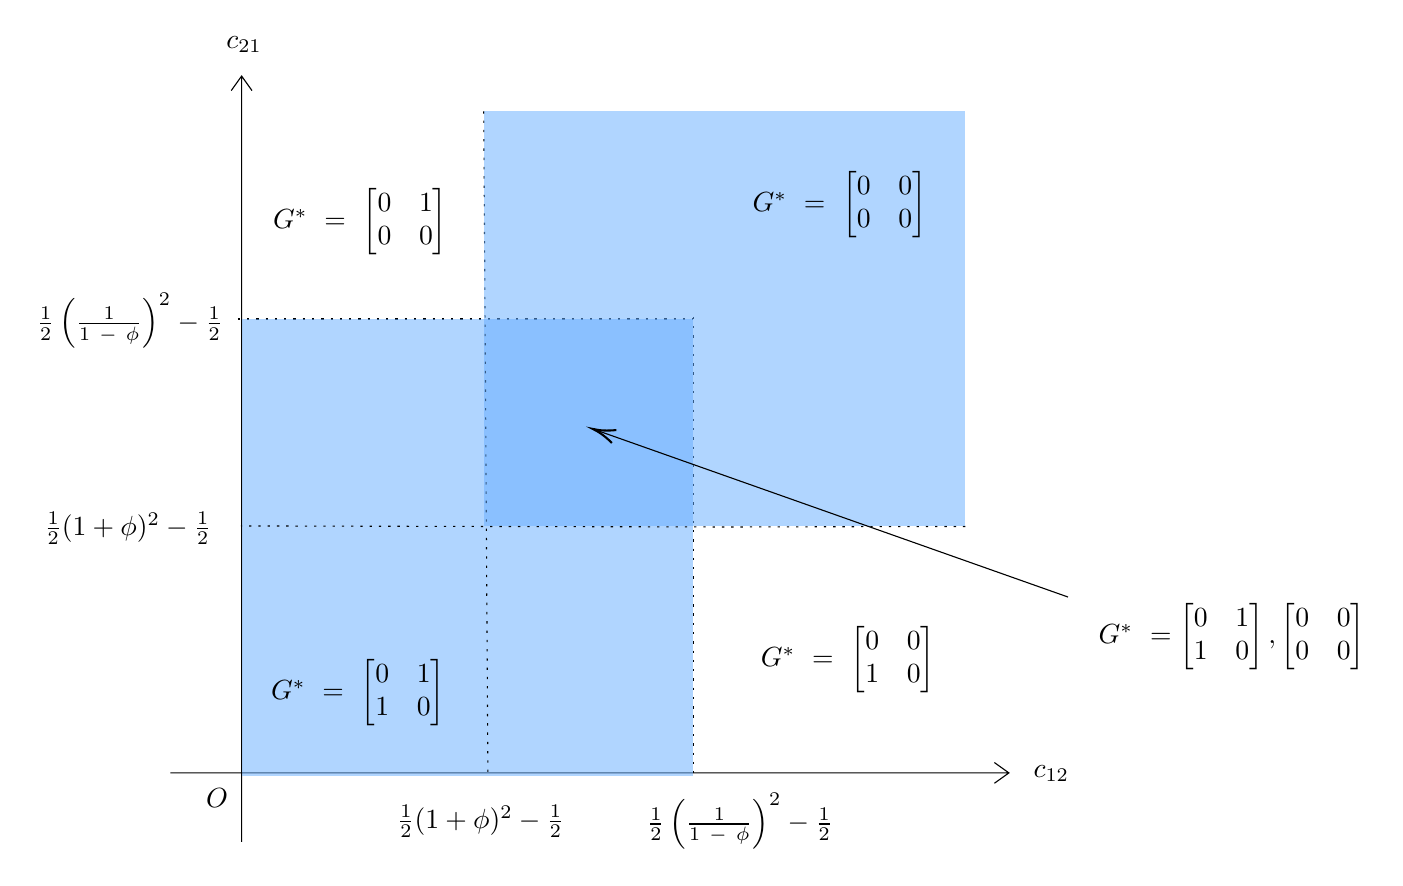
\begin{tikzpicture}[x=0.75pt,y=0.75pt,yscale=-1,xscale=1]
\draw  (115.49,390.74) -- (519.5,390.74)(149.83,55) -- (149.83,423.95) (512.5,385.74) -- (519.5,390.74) -- (512.5,395.74) (144.83,62) -- (149.83,55) -- (154.83,62)  ;
\draw [line width=0.75]  [dash pattern={on 0.84pt off 2.51pt}]  (148,172) -- (367.5,172) ;
\draw  [dash pattern={on 0.84pt off 2.51pt}]  (367.5,171) -- (367.5,392) ;
\draw  [draw opacity=0][fill={rgb, 255:red, 103; green, 174; blue, 255 }  ,fill opacity=0.52 ] (149.83,172) -- (367.5,172) -- (367.5,392) -- (149.83,392) -- cycle ;
\draw  [dash pattern={on 0.84pt off 2.51pt}]  (266.5,72) -- (268.5,392) ;
\draw  [dash pattern={on 0.84pt off 2.51pt}]  (498.5,272) -- (383.5,272.25) -- (149.5,271.75) ;
\draw  [draw opacity=0][fill={rgb, 255:red, 103; green, 174; blue, 255 }  ,fill opacity=0.52 ] (266.5,72) -- (498.5,72) -- (498.5,272) -- (266.5,272) -- cycle ;
\draw    (548,306) -- (320.89,225.67) ;
\draw [shift={(319,225)}, rotate = 379.48] [color={rgb, 255:red, 0; green, 0; blue, 0 }  ][line width=0.75]    (10.93,-3.29) .. controls (6.95,-1.4) and (3.31,-0.3) .. (0,0) .. controls (3.31,0.3) and (6.95,1.4) .. (10.93,3.29)   ;
\draw (540,391) node   {$c_{12}$};
\draw (151,40) node   {$c_{21}$};
\draw (138,403) node   {$O$};
\draw (96,173) node   {$\frac{1}{2}\left(\frac{1}{1\ -\ \phi }\right)^{2} -\frac{1}{2}$};
\draw (390,414) node   {$\frac{1}{2}\left(\frac{1}{1\ -\ \phi }\right)^{2} -\frac{1}{2}$};
\draw (95,273) node   {$\frac{1}{2}( 1+\phi )^{2} -\frac{1}{2}$};
\draw (265,414) node   {$\frac{1}{2}( 1+\phi )^{2} -\frac{1}{2}$};
\draw (438,117) node   {$G^{*} \ =\ \begin{bmatrix}
0 & 0\\
0 & 0
\end{bmatrix}$};
\draw (206,352) node   {$G^{*} \ =\ \begin{bmatrix}
0 & 1\\
1 & 0
\end{bmatrix}$};
\draw (207,125) node   {$G^{*} \ =\ \begin{bmatrix}
0 & 1\\
0 & 0
\end{bmatrix}$};
\draw (442,336) node   {$G^{*} \ =\ \begin{bmatrix}
0 & 0\\
1 & 0
\end{bmatrix}$};
\draw (627,325) node   {$G^{*} \ =\begin{bmatrix}
0 & 1\\
1 & 0
\end{bmatrix} ,\begin{bmatrix}
0 & 0\\
0 & 0
\end{bmatrix}$};
\end{tikzpicture}
\caption{Equilibrium network region} \label{fig:eq}
\end{figure}

Example 1 shows the equilibrium network may not be unique and Figure \ref{fig:eq} shows that the region of costs which brings the respective equilibrium network.
We can see the region which returns complete equilibrium network and empty equilibrium network overlap.
From this perspective, the algorithm can potentially converge multiple equilibria.
In each step, the number of the agents who do not take best responses is generally greater than one.
Therefore, the order of the agents who delete the links is changed, and the network in each steps is also changed.
This may lead to the different networks.

We focus on the greatest equilibrium network from now on, and denote it as $g^{**}$.
The greatest equilibrium can be obtained by designed best response dynamics algorithm.
Next algorithm returns the greatest equilibrium network.

\begin{algorithm}
\ 
\begin{description}
	\item[Step 0.]\mbox{}\\
		Let $g^{(0)}$ be the initial realized network where $g^{(0)} = g^p$, that is, chooosing strategy is $\psi_i^{(0)} \in \Psi_i$ such that $\psi_{ij}^{(0)} = 1$ for all $j \in N_i(g^p)$.
		Compute each players' optimal effort and payoffs.
		Denote the set of agents who do not take best response as $NB^{(0)}$:
		\begin{equation*}
		\begin{split}
			NB^{(0)} = \{i \in N &| \exists \tilde{\psi}_i \subset N_i(g^p) \ \text{s.t.} \ u_i(\bm{x}^*(g(\tilde{\psi}_1, \psi_{-i}^{(0)}), \tilde{\psi}_i, \psi_{-i}^{(0)}, \bm{C}, \phi) > u_i(\bm{x}^*(g(\bm{\psi}^{(0)})), \bm{\psi}^{(0)}, \bm{C}, \phi) \}
		\end{split}
		\end{equation*}
		Go into Step 1.
	\item[Step $k(\ge 1)$.]\mbox{}\\
		Check whether $NB^{(k-1)}$ is empty or not.

		If $NB^{(k-1)} = \emptyset$, define $g^* = g(\bm{\psi}^{(k-1)})$ and terminate the algorithm.

		Otherwise, choose a agent $i \in NB^{(k-1)}$ randomly.
		Agent $i$ takes best response, changing links, then new network is emerged.
		That is, $i$ changes her strategy from $\psi_i^{(k-1)}$ to $\psi_i^{(k)}$ such that $u_i(\bm{x}^*(g(\psi_i^{(k)}, \psi_{-i}^{(k-1)})), \psi_i^{(k)}, \psi_{-i}^{(k-1)}, \bm{C}, \phi) > u_i(\bm{x}^*(g(\bm{\psi}^{(k-1)})), \bm{\psi}^{(k-1)}, \bm{C}, \phi)$, and for any other agents $j (\neq i)$ remain their strategies, $\psi_j^{(k)} = \psi_j^{(k-1)}$.
		If agent $i$ has multiple such strategies, choose largest one.
		Then, new network $g(\bm{\psi}^{(k)})$ is realized.
		Compute each players' payoffs and define $NB^{(k)}$:
		\begin{equation*}
		\begin{split}
			NB^{(k)} = \{i \in N &| \exists \tilde{\psi}_i \subset N_i(g^p) \ \text{s.t.} \ u_i(\bm{x}^*(g(\tilde{\psi}_1, \psi_{-i}^{(k)}), \tilde{\psi}_i, \psi_{-i}^{(k)}, \bm{C}, \phi) > u_i(\bm{x}^*(g(\bm{\psi}^{(k)})), \bm{\psi}^{(k)}, \bm{C}, \phi) \}
		\end{split}
		\end{equation*}
		Proceed to Step $k+1$.
\end{description}
\end{algorithm}

Algorithm 1 is one of the {\it{best response dynamics}} algorithms, where agents take their best reponses in each steps.
In the algorithm, agent choose largest strategy if she has multiple best responses.
We have to show that there always exists the largest best response.
Next lemma shows its existence.

\begin{lemma}
In Algorithm 1, for any step $k$, $|BR_i(\psi_{-i}^{(k-1)})| = 1$ for any $i \in NB^{(k-1)}$
\end{lemma}

By this lemma, we can see Algotihm 1 works well.
You notice that if the best reponse dynamics halts, it returns a pure strategy Nash equilibrium.\footnote{See Nisan, Noam, et al.~\cite{AGT}}
As in Topkis (1998)~\cite{topkis1998}, returned network is the greatest equilibrium network.


\subsection{Comparative Statics}

In this section, we argue the comparative statics by changing the parameter $\bm{C}$.
When the cost of forming links decrease, we conjecture that the network becomes denser because agents are more likely to form the links.

We denote that, for network $g$ and $h$, $g \supseteq h$ if all links in the network $h$ are existed in the network $g$, that is $\bm{G} \ge \bm{H}$.
Next proposition shows that our conjection is verified.
This result is based on the supermodularity of 1st stage game.

\begin{proposition}
Given the potential network $g^p$.
Consider the cost $\bm{\hat{C}}$ and $\bm{C}$ with $\bm{\hat{C}} \le \bm{C}$.
Then,
\[ g^{**}(\bm{\psi}^*(g^p, \bm{\hat{C}}, \phi, \bm{\alpha})) \supseteq g^{**}(\bm{\psi}^*(g^p, \bm{C}, \phi, \bm{\alpha})) \]
\end{proposition}

By the same argument, we have the following corollary.

\begin{corollary}
	Given the potential network $g^p$. For $\hat{\phi} \ge \phi$ which satisfy the Assumption,
        \[ g^{**}(\bm{\psi}^*(g^p, \bm{C}, \hat{\phi}, \bm{\alpha})) \supseteq g^{**}(\bm{\psi}^*(g^p, \bm{C}, \phi, \bm{\alpha})) \]
    For $\bm{\hat{\alpha}} \ge \bm{\alpha}$,
        \[ g^{**}(\bm{\psi}^*(g^p, \bm{C}, \phi, \bm{\hat{\alpha}})) \supseteq g^{**}(\bm{\psi}^*(g^p, \bm{C}, \phi, \bm{\alpha})) \]
\end{corollary}

The realized network is a increasing function in the costs of forming links.
However, it is obvious that this function is discontiunous.
The next example shows that small changes in the costs makes the network entirely changed.

\begin{example}
Consider the network with $n = 5$, and the potential network so that $g_{ij}^p = 1$ for any pair $ij(i \neq j)$.
Assume $\bm{\alpha} = (1, 1, 1, 1, 1)$ and $\phi = \frac{1}{5}$, which satisfies the Assumption 1.
Consider the costs $\bm{C}$ such that
\[ \bm{C} = \left[
			\begin{array}{ccccc}
				0 & 3 & 3 & 3 & 3 \\
				3 & 0 & 3 & 3 & 3 \\
				3 & 3 & 0 & 3 & 3 \\
				3 & 3 & 3 & 0 & 3  \\
				3 & 3 & 3 & 3 & 0
			\end{array} \right] \]
Then, the equilibrium network $g^*$ becomes
\[\bm{G}^{**} = \left[
			\begin{array}{ccccc}
				0 & 1 & 1 & 1 & 1 \\
				1 & 0 & 1 & 1 & 1 \\
				1 & 1 & 0 & 1 & 1 \\
				1 & 1 & 1 & 0 & 1 \\
				1 & 1 & 1 & 1 & 0
			\end{array} \right] \]
The equilibrium network becomes complete network.
On the other hand, when the cost of forming a link from agent $1$ to agent $2$ slightly increases, for small enough $\epsilon > 0$,
\[ \bm{\hat{C}} = \left[
			\begin{array}{ccccc}
				0 & 3 + \epsilon & 3 & 3 & 3 \\
				3 & 0 & 3 & 3 & 3 \\
				3 & 3 & 0 & 3 & 3 \\
				3 & 3 & 3 & 0 & 3  \\
				3 & 3 & 3 & 3 & 0
			\end{array} \right] \]
then, the equilibrium network $\hat{g}^*$ becomes
\[ \bm{\hat{G}}^{**} = \left[
			\begin{array}{ccccc}
				0 & 0 & 0 & 0 & 0 \\
				0 & 0 & 0 & 0 & 0 \\
				0 & 0 & 0 & 0 & 0 \\
				0 & 0 & 0 & 0 & 0 \\
				0 & 0 & 0 & 0 & 0
			\end{array} \right] \]
The equilibrium network is empty network.
\end{example}


%% The picture of equilibrium
\begin{figure}[h]
\centering
\tikzset{every picture/.style={line width=0.75pt}}        
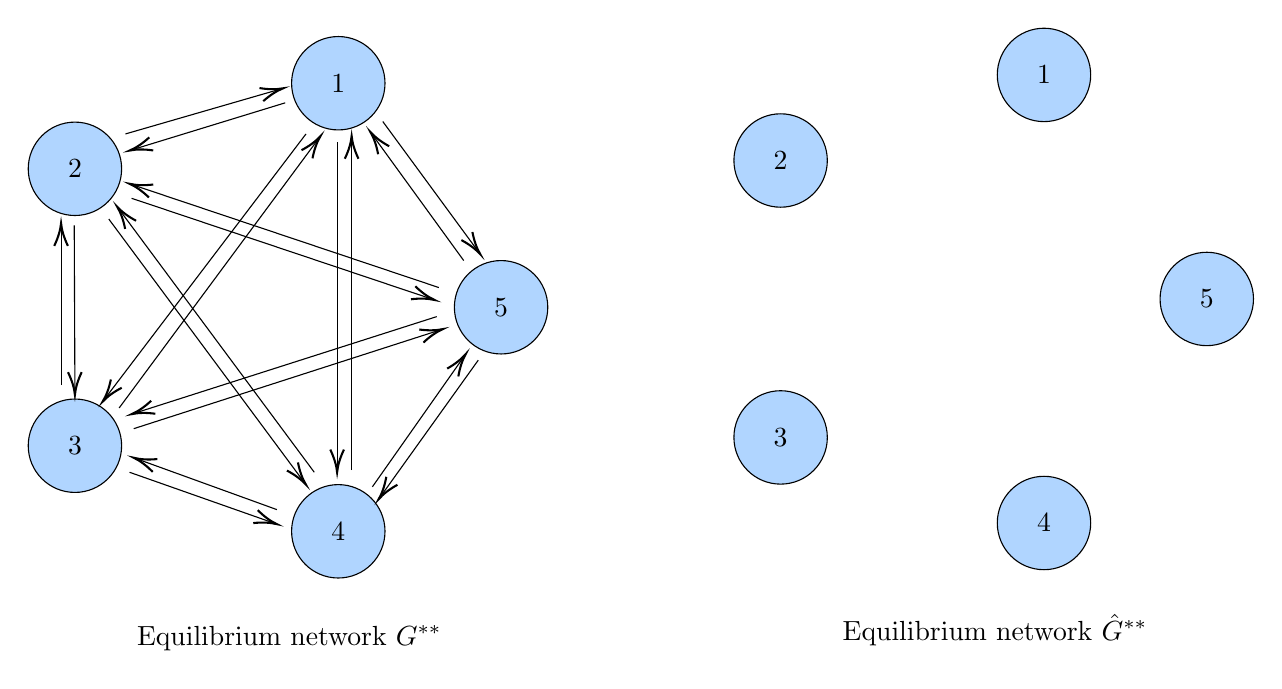
\begin{tikzpicture}[x=0.75pt,y=0.75pt,yscale=-1,xscale=1]
\draw  [fill={rgb, 255:red, 103; green, 174; blue, 255 }  ,fill opacity=0.52 ] (199.07,64.56) .. controls (199.07,52.13) and (209.15,42.06) .. (221.57,42.06) .. controls (234,42.06) and (244.07,52.13) .. (244.07,64.56) .. controls (244.07,76.98) and (234,87.06) .. (221.57,87.06) .. controls (209.15,87.06) and (199.07,76.98) .. (199.07,64.56) -- cycle ;
\draw  [fill={rgb, 255:red, 103; green, 174; blue, 255 }  ,fill opacity=0.52 ] (72.18,105.79) .. controls (72.18,93.36) and (82.25,83.29) .. (94.68,83.29) .. controls (107.1,83.29) and (117.18,93.36) .. (117.18,105.79) .. controls (117.18,118.21) and (107.1,128.29) .. (94.68,128.29) .. controls (82.25,128.29) and (72.18,118.21) .. (72.18,105.79) -- cycle ;
\draw  [fill={rgb, 255:red, 103; green, 174; blue, 255 }  ,fill opacity=0.52 ] (277.5,172.5) .. controls (277.5,160.07) and (287.57,150) .. (300,150) .. controls (312.43,150) and (322.5,160.07) .. (322.5,172.5) .. controls (322.5,184.93) and (312.43,195) .. (300,195) .. controls (287.57,195) and (277.5,184.93) .. (277.5,172.5) -- cycle ;
\draw  [fill={rgb, 255:red, 103; green, 174; blue, 255 }  ,fill opacity=0.52 ] (72.18,239.21) .. controls (72.18,226.79) and (82.25,216.71) .. (94.68,216.71) .. controls (107.1,216.71) and (117.18,226.79) .. (117.18,239.21) .. controls (117.18,251.64) and (107.1,261.71) .. (94.68,261.71) .. controls (82.25,261.71) and (72.18,251.64) .. (72.18,239.21) -- cycle ;
\draw  [fill={rgb, 255:red, 103; green, 174; blue, 255 }  ,fill opacity=0.52 ] (199.07,280.44) .. controls (199.07,268.02) and (209.15,257.94) .. (221.57,257.94) .. controls (234,257.94) and (244.07,268.02) .. (244.07,280.44) .. controls (244.07,292.87) and (234,302.94) .. (221.57,302.94) .. controls (209.15,302.94) and (199.07,292.87) .. (199.07,280.44) -- cycle ;
\draw    (196,74) -- (122.91,96.41) ;
\draw [shift={(121,97)}, rotate = 342.95] [color={rgb, 255:red, 0; green, 0; blue, 0 }  ][line width=0.75]    (10.93,-3.29) .. controls (6.95,-1.4) and (3.31,-0.3) .. (0,0) .. controls (3.31,0.3) and (6.95,1.4) .. (10.93,3.29)   ;
\draw    (221,93) -- (221,250) ;
\draw [shift={(221,252)}, rotate = 270] [color={rgb, 255:red, 0; green, 0; blue, 0 }  ][line width=0.75]    (10.93,-3.29) .. controls (6.95,-1.4) and (3.31,-0.3) .. (0,0) .. controls (3.31,0.3) and (6.95,1.4) .. (10.93,3.29)   ;
\draw    (119,89) -- (193.08,67.56) ;
\draw [shift={(195,67)}, rotate = 523.86] [color={rgb, 255:red, 0; green, 0; blue, 0 }  ][line width=0.75]    (10.93,-3.29) .. controls (6.95,-1.4) and (3.31,-0.3) .. (0,0) .. controls (3.31,0.3) and (6.95,1.4) .. (10.93,3.29)   ;
\draw    (111,130) -- (204.81,256.39) ;
\draw [shift={(206,258)}, rotate = 233.42000000000002] [color={rgb, 255:red, 0; green, 0; blue, 0 }  ][line width=0.75]    (10.93,-3.29) .. controls (6.95,-1.4) and (3.31,-0.3) .. (0,0) .. controls (3.31,0.3) and (6.95,1.4) .. (10.93,3.29)   ;
\draw    (121,252) -- (190.11,276.34) ;
\draw [shift={(192,277)}, rotate = 199.4] [color={rgb, 255:red, 0; green, 0; blue, 0 }  ][line width=0.75]    (10.93,-3.29) .. controls (6.95,-1.4) and (3.31,-0.3) .. (0,0) .. controls (3.31,0.3) and (6.95,1.4) .. (10.93,3.29)   ;
\draw    (238,259) -- (281.85,196.64) ;
\draw [shift={(283,195)}, rotate = 485.11] [color={rgb, 255:red, 0; green, 0; blue, 0 }  ][line width=0.75]    (10.93,-3.29) .. controls (6.95,-1.4) and (3.31,-0.3) .. (0,0) .. controls (3.31,0.3) and (6.95,1.4) .. (10.93,3.29)   ;
\draw    (243,83) -- (288.82,145.39) ;
\draw [shift={(290,147)}, rotate = 233.71] [color={rgb, 255:red, 0; green, 0; blue, 0 }  ][line width=0.75]    (10.93,-3.29) .. controls (6.95,-1.4) and (3.31,-0.3) .. (0,0) .. controls (3.31,0.3) and (6.95,1.4) .. (10.93,3.29)   ;
\draw    (206,89) -- (109.21,216.41) ;
\draw [shift={(108,218)}, rotate = 307.22] [color={rgb, 255:red, 0; green, 0; blue, 0 }  ][line width=0.75]    (10.93,-3.29) .. controls (6.95,-1.4) and (3.31,-0.3) .. (0,0) .. controls (3.31,0.3) and (6.95,1.4) .. (10.93,3.29)   ;
\draw    (94.35,133) -- (94.67,212.71) ;
\draw [shift={(94.68,214.71)}, rotate = 269.77] [color={rgb, 255:red, 0; green, 0; blue, 0 }  ][line width=0.75]    (10.93,-3.29) .. controls (6.95,-1.4) and (3.31,-0.3) .. (0,0) .. controls (3.31,0.3) and (6.95,1.4) .. (10.93,3.29)   ;
\draw    (122,120) -- (266.1,168.36) ;
\draw [shift={(268,169)}, rotate = 198.55] [color={rgb, 255:red, 0; green, 0; blue, 0 }  ][line width=0.75]    (10.93,-3.29) .. controls (6.95,-1.4) and (3.31,-0.3) .. (0,0) .. controls (3.31,0.3) and (6.95,1.4) .. (10.93,3.29)   ;
\draw    (116,221) -- (211.81,91.61) ;
\draw [shift={(213,90)}, rotate = 486.52] [color={rgb, 255:red, 0; green, 0; blue, 0 }  ][line width=0.75]    (10.93,-3.29) .. controls (6.95,-1.4) and (3.31,-0.3) .. (0,0) .. controls (3.31,0.3) and (6.95,1.4) .. (10.93,3.29)   ;
\draw    (88,210) -- (88,134) ;
\draw [shift={(88,132)}, rotate = 450] [color={rgb, 255:red, 0; green, 0; blue, 0 }  ][line width=0.75]    (10.93,-3.29) .. controls (6.95,-1.4) and (3.31,-0.3) .. (0,0) .. controls (3.31,0.3) and (6.95,1.4) .. (10.93,3.29)   ;
\draw    (123,231) -- (270.1,183.61) ;
\draw [shift={(272,183)}, rotate = 522.14] [color={rgb, 255:red, 0; green, 0; blue, 0 }  ][line width=0.75]    (10.93,-3.29) .. controls (6.95,-1.4) and (3.31,-0.3) .. (0,0) .. controls (3.31,0.3) and (6.95,1.4) .. (10.93,3.29)   ;
\draw    (228,251) -- (228,92) ;
\draw [shift={(228,90)}, rotate = 450] [color={rgb, 255:red, 0; green, 0; blue, 0 }  ][line width=0.75]    (10.93,-3.29) .. controls (6.95,-1.4) and (3.31,-0.3) .. (0,0) .. controls (3.31,0.3) and (6.95,1.4) .. (10.93,3.29)   ;
\draw    (116.19,125.61) -- (210,252) ;
\draw [shift={(115,124)}, rotate = 53.42] [color={rgb, 255:red, 0; green, 0; blue, 0 }  ][line width=0.75]    (10.93,-3.29) .. controls (6.95,-1.4) and (3.31,-0.3) .. (0,0) .. controls (3.31,0.3) and (6.95,1.4) .. (10.93,3.29)   ;
\draw    (192,270) -- (124.88,245.68) ;
\draw [shift={(123,245)}, rotate = 379.91999999999996] [color={rgb, 255:red, 0; green, 0; blue, 0 }  ][line width=0.75]    (10.93,-3.29) .. controls (6.95,-1.4) and (3.31,-0.3) .. (0,0) .. controls (3.31,0.3) and (6.95,1.4) .. (10.93,3.29)   ;
\draw    (282,150) -- (238.17,89.62) ;
\draw [shift={(237,88)}, rotate = 414.03] [color={rgb, 255:red, 0; green, 0; blue, 0 }  ][line width=0.75]    (10.93,-3.29) .. controls (6.95,-1.4) and (3.31,-0.3) .. (0,0) .. controls (3.31,0.3) and (6.95,1.4) .. (10.93,3.29)   ;
\draw    (270,163) -- (122.9,113.64) ;
\draw [shift={(121,113)}, rotate = 378.55] [color={rgb, 255:red, 0; green, 0; blue, 0 }  ][line width=0.75]    (10.93,-3.29) .. controls (6.95,-1.4) and (3.31,-0.3) .. (0,0) .. controls (3.31,0.3) and (6.95,1.4) .. (10.93,3.29)   ;
\draw    (269,177) -- (123.9,223.39) ;
\draw [shift={(122,224)}, rotate = 342.27] [color={rgb, 255:red, 0; green, 0; blue, 0 }  ][line width=0.75]    (10.93,-3.29) .. controls (6.95,-1.4) and (3.31,-0.3) .. (0,0) .. controls (3.31,0.3) and (6.95,1.4) .. (10.93,3.29)   ;
\draw    (289,198) -- (242.16,263.37) ;
\draw [shift={(241,265)}, rotate = 305.62] [color={rgb, 255:red, 0; green, 0; blue, 0 }  ][line width=0.75]    (10.93,-3.29) .. controls (6.95,-1.4) and (3.31,-0.3) .. (0,0) .. controls (3.31,0.3) and (6.95,1.4) .. (10.93,3.29)   ;
\draw  [fill={rgb, 255:red, 103; green, 174; blue, 255 }  ,fill opacity=0.52 ] (539.07,60.56) .. controls (539.07,48.13) and (549.15,38.06) .. (561.57,38.06) .. controls (574,38.06) and (584.07,48.13) .. (584.07,60.56) .. controls (584.07,72.98) and (574,83.06) .. (561.57,83.06) .. controls (549.15,83.06) and (539.07,72.98) .. (539.07,60.56) -- cycle ;
\draw  [fill={rgb, 255:red, 103; green, 174; blue, 255 }  ,fill opacity=0.52 ] (412.18,101.79) .. controls (412.18,89.36) and (422.25,79.29) .. (434.68,79.29) .. controls (447.1,79.29) and (457.18,89.36) .. (457.18,101.79) .. controls (457.18,114.21) and (447.1,124.29) .. (434.68,124.29) .. controls (422.25,124.29) and (412.18,114.21) .. (412.18,101.79) -- cycle ;
\draw  [fill={rgb, 255:red, 103; green, 174; blue, 255 }  ,fill opacity=0.52 ] (617.5,168.5) .. controls (617.5,156.07) and (627.57,146) .. (640,146) .. controls (652.43,146) and (662.5,156.07) .. (662.5,168.5) .. controls (662.5,180.93) and (652.43,191) .. (640,191) .. controls (627.57,191) and (617.5,180.93) .. (617.5,168.5) -- cycle ;
\draw  [fill={rgb, 255:red, 103; green, 174; blue, 255 }  ,fill opacity=0.52 ] (412.18,235.21) .. controls (412.18,222.79) and (422.25,212.71) .. (434.68,212.71) .. controls (447.1,212.71) and (457.18,222.79) .. (457.18,235.21) .. controls (457.18,247.64) and (447.1,257.71) .. (434.68,257.71) .. controls (422.25,257.71) and (412.18,247.64) .. (412.18,235.21) -- cycle ;
\draw  [fill={rgb, 255:red, 103; green, 174; blue, 255 }  ,fill opacity=0.52 ] (539.07,276.44) .. controls (539.07,264.02) and (549.15,253.94) .. (561.57,253.94) .. controls (574,253.94) and (584.07,264.02) .. (584.07,276.44) .. controls (584.07,288.87) and (574,298.94) .. (561.57,298.94) .. controls (549.15,298.94) and (539.07,288.87) .. (539.07,276.44) -- cycle ;
\draw (221.57,64.56) node   {$1$};
\draw (94.68,105.79) node   {$2$};
\draw (94.68,239.21) node   {$3$};
\draw (221.57,280.44) node   {$4$};
\draw (300,172.5) node   {$5$};
\draw (198,332) node  [align=left] {Equilibrium network $\displaystyle G^{**}$};
\draw (561.57,60.56) node   {$1$};
\draw (434.68,101.79) node   {$2$};
\draw (434.68,235.21) node   {$3$};
\draw (561.57,276.44) node   {$4$};
\draw (640,168.5) node   {$5$};
\draw (538,328) node  [align=left] {Equilibrium network $\displaystyle \hat{G}^{**}$};
\end{tikzpicture}
\caption{Equilibrium networks in Example 2} \label{fig:ex2}
\end{figure}

With the cost structure $\bm{C}$, all agents keep connected to all other agents, but all agents are on the threshhold from keeping all links to removing them.
In fact, all agents are indifference between them, keeping all links and removing all links give the exactly same payoff.
Algorithm 1 returns the complete networks by its construction.
When the cost of forming link from agent 1 to agent 2 slightly increases, agent 1 does not keep links to the others because agent 1's gain from agent 2 cannot compensate its cost.
Since agent 1 removes all links, agent 1's level of effort drastically diclines.
The gain from agent 1 also declines, and the levels of effort of agents declines.
Therefore, the benefit of forming links cannot compensate the cost of keeping links, and all agents remove all links.

We can see tiny changes in the costs generates large discontinuity in the structure of the network.
Example 2 shows that our model incorporates the {\it{phase transition}}: the phenomenon that the feature of the network is totally changed\footnote{see Jackson(2010)~\cite{social}}.
But as discussed above, it is difficult to identify the threshold of the transition by the discontinuity of the realized network.


\section{Policy implication}

\subsection{Key player policy}

We first argue the {\it{key player}} in the network, who has the largest impact on the aggregate behavior of the network.
In the previous literatures, for example Ballester, Calvo-Armengol, and Zenou(2006, 2010)~\cite{whowho, delinquent} and Liu et.al.(2012)~\cite{criminal}, argue the key player and give necessary and sufficient condition of who becomes it in the context of similar model\footnote{Denbee, Julliard, Li, and Yuan(2018)~\cite{denbee} defines the key player in financial network}.
In these papers, key player is defined as the agent who, once removed from the network, generates the highest possible reduction in aggreate effort level.
Key player is thought of, for example, the player who supports the criminal activity of his friends in the context of criminal network.
The formal definition of key player is given as follows:

\begin{definition}
Agent $i$ is the {\it{key player in exogenous network}} if, given network $g$,
\[ i \in \arg \max_{i \in N} \{ x^*(g) - x^*(g^{-i}) \} \]
\end{definition}

Here we denote $x^*(g) = \sum_{i=1}^n x_i^*(g)$ and $g^{-i}$ is the network where agent $i$ is removed from the network $g$.
The adjecency matrix of $g^{-i}$, $\bm{G}^{-i}$, is obtained from $\bm{G}$ by setting to zero all of its $i$th row and column entries.
Previous literatures show the key player in exogenous network does not always coincide with the most active player who excerts highest effort.

In this paper, the definition of key player might be different from the previous ones.
Since the network is endogenous in our model, the key player is the agent who generates the largest reduction in the total effort level once she is removed from the potential network.

\begin{definition}
Agent $i$ is the {\it{key player in endogenous network}} if, given potential network $g^p$,
\[ i \in \arg \max_{i \in N} \{ x^*(g(\bm{\psi}({g^p}^{-i}, \bm{C}))) - x^*(g(\bm{\psi}({g^p}^{-i}, \bm{C}^{-i}))) \} \]
\end{definition}
Here we denote ${g^p}^{-i}$ is the network where agent $i$ is removed from the network $g^p$ as before.
$\bm{C}^{-i}$ is obtained from $\bm{C}$ by setting to zero all of its $i$th row and column entries.

As discussed in the previous section, there exists a discontinuity of the network realization in the link formation costs, so it is very difficult to identify the condition to be a key player\footnote{Similar to Elliott, Golub, and Jackson(2014)~\cite{contagion}, we cannot identify which banks will be in default by the discontinuity of banks' values}.
The realization of the network is a key factor to be a key player in the endogenous network.
We know that denser network leads higher effort level by the network externality, so, in order to become a key player in endogenous network, the realized network after removing should be sparse.

Although it is difficult to identify who becomes key player, we can find that the most active player, key player in endogenous network, and key player in exogenous network can be different each other.
To compare the kay player in endogenous network and exogenous network, we treat realized network from the potential network and costs as given, then compute the key player in exogenous network.
Endogenous one is computed by the definition.

\begin{example}
Consider the network with $n=5$, and the potential network so that $g_{ij}^p = 1$ for any pair $ij(i \neq j)$.
Assume $\bm{\alpha} = (1, 1, 1, 1, 1)$ and $\phi = \frac{1}{5}$, which satisfies the Assumption 1.

Consider the link formation costs as follows:
\[\bm{C} = \left[
			\begin{array}{ccccc}
				0 & 3.6 & 0.2 & 0.2 & 0.2 \\
				0.3 & 0 & 0.2 & 0.5 & 5.5 \\
				0.2 & 0.2 & 0 & 4.5 & 4.3 \\
				4.1 & 0.2 & 0.4 & 0 & 6.5 \\
				3.2 & 4.1 & 0.3 & 1.0 & 0
			\end{array} \right] \]
Then, the realized equilibrium network $g^*$ is:
\[\bm{G}^* = \left[
			\begin{array}{ccccc}
				0 & 0 & 1 & 1 & 1 \\
				1 & 0 & 1 & 1 & 0 \\
				1 & 1 & 0 & 0 & 0 \\
				0 & 1 & 1 & 0 & 0 \\
				0 & 0 & 1 & 0 & 0
			\end{array} \right] \]
In this network, we can compute the equilibrium effort levels by computer.
\[ (x_1^*, x_2^*, x_3^*, x_4^*, x_5^*) \approx (1.99541284, 2.12155963, 1.8233945, 1.78899083, 1.3646789) \]
As you see, the agent who excerts highest effort is agent $2$.
However, the key player in endogenous network $g^*$ is agent $1$.
On the other hand, when we treat the network $g^*$ as given, the key player in exogenous network is agent $3$.
See Table \ref{tab:key player}.
Figure \ref{fig:ex3} shows the key player in endogenous and exogenous network in this example.

\begin{table}[htb]
  \begin{center}
    \begin{tabular}{|l|c|} \hline
      agent with highest effort & agent $2$ \\ \hline
      key player in endogenous network & agent $1$ \\ \hline
      key player in exogenous network & agent $3$ \\ \hline
    \end{tabular}
    \caption{Difference of key players}
    \label{tab:key player}
  \end{center}
\end{table}
\end{example}


%% The picture of key players
\begin{figure}[h]
\raggedleft
\tikzset{every picture/.style={line width=0.75pt}}      
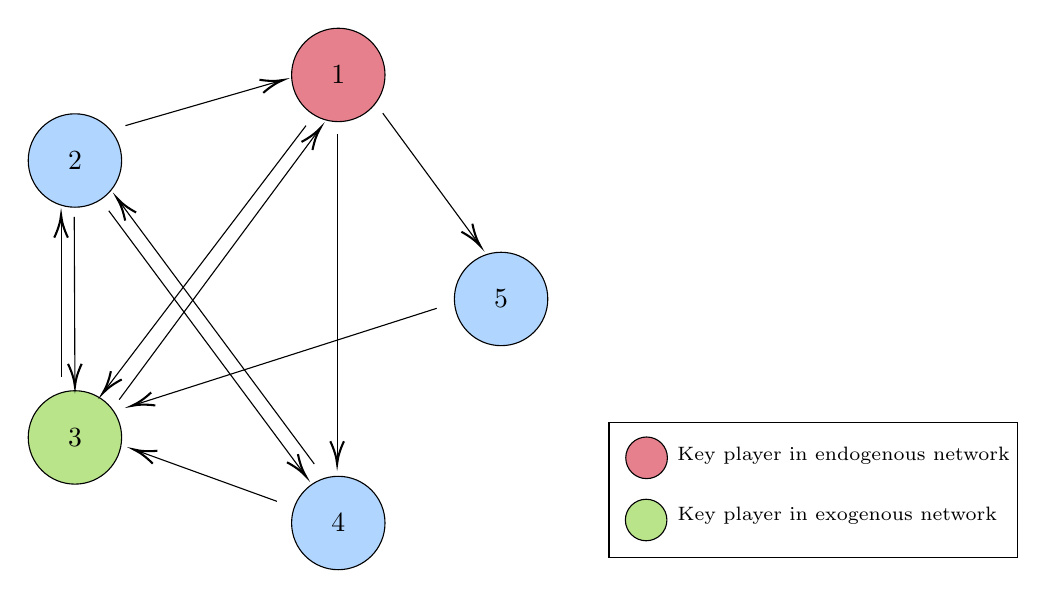
\begin{tikzpicture}[x=0.75pt,y=0.75pt,yscale=-1,xscale=1]
\draw  [fill={rgb, 255:red, 208; green, 2; blue, 27 }  ,fill opacity=0.5 ] (416.07,67.56) .. controls (416.07,55.13) and (426.15,45.06) .. (438.57,45.06) .. controls (451,45.06) and (461.07,55.13) .. (461.07,67.56) .. controls (461.07,79.98) and (451,90.06) .. (438.57,90.06) .. controls (426.15,90.06) and (416.07,79.98) .. (416.07,67.56) -- cycle ;
\draw  [fill={rgb, 255:red, 103; green, 174; blue, 255 }  ,fill opacity=0.52 ] (289.18,108.79) .. controls (289.18,96.36) and (299.25,86.29) .. (311.68,86.29) .. controls (324.1,86.29) and (334.18,96.36) .. (334.18,108.79) .. controls (334.18,121.21) and (324.1,131.29) .. (311.68,131.29) .. controls (299.25,131.29) and (289.18,121.21) .. (289.18,108.79) -- cycle ;
\draw  [fill={rgb, 255:red, 103; green, 174; blue, 255 }  ,fill opacity=0.52 ] (494.5,175.5) .. controls (494.5,163.07) and (504.57,153) .. (517,153) .. controls (529.43,153) and (539.5,163.07) .. (539.5,175.5) .. controls (539.5,187.93) and (529.43,198) .. (517,198) .. controls (504.57,198) and (494.5,187.93) .. (494.5,175.5) -- cycle ;
\draw  [fill={rgb, 255:red, 115; green, 201; blue, 21 }  ,fill opacity=0.5 ] (289.18,242.21) .. controls (289.18,229.79) and (299.25,219.71) .. (311.68,219.71) .. controls (324.1,219.71) and (334.18,229.79) .. (334.18,242.21) .. controls (334.18,254.64) and (324.1,264.71) .. (311.68,264.71) .. controls (299.25,264.71) and (289.18,254.64) .. (289.18,242.21) -- cycle ;
\draw  [fill={rgb, 255:red, 103; green, 174; blue, 255 }  ,fill opacity=0.52 ] (416.07,283.44) .. controls (416.07,271.02) and (426.15,260.94) .. (438.57,260.94) .. controls (451,260.94) and (461.07,271.02) .. (461.07,283.44) .. controls (461.07,295.87) and (451,305.94) .. (438.57,305.94) .. controls (426.15,305.94) and (416.07,295.87) .. (416.07,283.44) -- cycle ;
\draw    (438,96) -- (438,253) ;
\draw [shift={(438,255)}, rotate = 270] [color={rgb, 255:red, 0; green, 0; blue, 0 }  ][line width=0.75]    (10.93,-3.29) .. controls (6.95,-1.4) and (3.31,-0.3) .. (0,0) .. controls (3.31,0.3) and (6.95,1.4) .. (10.93,3.29)   ;
\draw    (336,92) -- (410.08,70.56) ;
\draw [shift={(412,70)}, rotate = 523.86] [color={rgb, 255:red, 0; green, 0; blue, 0 }  ][line width=0.75]    (10.93,-3.29) .. controls (6.95,-1.4) and (3.31,-0.3) .. (0,0) .. controls (3.31,0.3) and (6.95,1.4) .. (10.93,3.29)   ;
\draw    (328,133) -- (421.81,259.39) ;
\draw [shift={(423,261)}, rotate = 233.42000000000002] [color={rgb, 255:red, 0; green, 0; blue, 0 }  ][line width=0.75]    (10.93,-3.29) .. controls (6.95,-1.4) and (3.31,-0.3) .. (0,0) .. controls (3.31,0.3) and (6.95,1.4) .. (10.93,3.29)   ;
\draw    (460,86) -- (505.82,148.39) ;
\draw [shift={(507,150)}, rotate = 233.71] [color={rgb, 255:red, 0; green, 0; blue, 0 }  ][line width=0.75]    (10.93,-3.29) .. controls (6.95,-1.4) and (3.31,-0.3) .. (0,0) .. controls (3.31,0.3) and (6.95,1.4) .. (10.93,3.29)   ;
\draw    (423,92) -- (326.21,219.41) ;
\draw [shift={(325,221)}, rotate = 307.22] [color={rgb, 255:red, 0; green, 0; blue, 0 }  ][line width=0.75]    (10.93,-3.29) .. controls (6.95,-1.4) and (3.31,-0.3) .. (0,0) .. controls (3.31,0.3) and (6.95,1.4) .. (10.93,3.29)   ;
\draw    (311.35,136) -- (311.67,215.71) ;
\draw [shift={(311.68,217.71)}, rotate = 269.77] [color={rgb, 255:red, 0; green, 0; blue, 0 }  ][line width=0.75]    (10.93,-3.29) .. controls (6.95,-1.4) and (3.31,-0.3) .. (0,0) .. controls (3.31,0.3) and (6.95,1.4) .. (10.93,3.29)   ;
\draw    (333,224) -- (428.81,94.61) ;
\draw [shift={(430,93)}, rotate = 486.52] [color={rgb, 255:red, 0; green, 0; blue, 0 }  ][line width=0.75]    (10.93,-3.29) .. controls (6.95,-1.4) and (3.31,-0.3) .. (0,0) .. controls (3.31,0.3) and (6.95,1.4) .. (10.93,3.29)   ;
\draw    (305,213) -- (305,137) ;
\draw [shift={(305,135)}, rotate = 450] [color={rgb, 255:red, 0; green, 0; blue, 0 }  ][line width=0.75]    (10.93,-3.29) .. controls (6.95,-1.4) and (3.31,-0.3) .. (0,0) .. controls (3.31,0.3) and (6.95,1.4) .. (10.93,3.29)   ;
\draw    (333.19,128.61) -- (427,255) ;
\draw [shift={(332,127)}, rotate = 53.42] [color={rgb, 255:red, 0; green, 0; blue, 0 }  ][line width=0.75]    (10.93,-3.29) .. controls (6.95,-1.4) and (3.31,-0.3) .. (0,0) .. controls (3.31,0.3) and (6.95,1.4) .. (10.93,3.29)   ;
\draw    (409,273) -- (341.88,248.68) ;
\draw [shift={(340,248)}, rotate = 379.91999999999996] [color={rgb, 255:red, 0; green, 0; blue, 0 }  ][line width=0.75]    (10.93,-3.29) .. controls (6.95,-1.4) and (3.31,-0.3) .. (0,0) .. controls (3.31,0.3) and (6.95,1.4) .. (10.93,3.29)   ;
\draw    (486,180) -- (340.9,226.39) ;
\draw [shift={(339,227)}, rotate = 342.27] [color={rgb, 255:red, 0; green, 0; blue, 0 }  ][line width=0.75]    (10.93,-3.29) .. controls (6.95,-1.4) and (3.31,-0.3) .. (0,0) .. controls (3.31,0.3) and (6.95,1.4) .. (10.93,3.29)   ;
\draw   (569,235) -- (766,235) -- (766,300) -- (569,300) -- cycle ;
\draw  [fill={rgb, 255:red, 208; green, 2; blue, 27 }  ,fill opacity=0.5 ] (577.07,252.03) .. controls (577.07,246.49) and (581.56,242) .. (587.1,242) .. controls (592.64,242) and (597.13,246.49) .. (597.13,252.03) .. controls (597.13,257.57) and (592.64,262.06) .. (587.1,262.06) .. controls (581.56,262.06) and (577.07,257.57) .. (577.07,252.03) -- cycle ;
\draw  [fill={rgb, 255:red, 115; green, 201; blue, 21 }  ,fill opacity=0.5 ] (576.89,282) .. controls (576.89,276.48) and (581.37,272) .. (586.89,272) .. controls (592.41,272) and (596.89,276.48) .. (596.89,282) .. controls (596.89,287.52) and (592.41,292) .. (586.89,292) .. controls (581.37,292) and (576.89,287.52) .. (576.89,282) -- cycle ;
\draw (438.57,67.56) node   {$1$};
\draw (311.68,108.79) node   {$2$};
\draw (311.68,242.21) node   {$3$};
\draw (438.57,283.44) node   {$4$};
\draw (517,175.5) node   {$5$};
\draw (682,251) node  [align=left] {{\scriptsize Key player in endogenous network}};
\draw (679,280) node  [align=left] {{\scriptsize Key player in exogenous network}};
\end{tikzpicture}
\caption{Equilibrium network $G^{*}$ and key players in Example 3} \label{fig:ex3}
\end{figure}

Agent 2 is the most active player (with highest effort) in both endogenous and exogenous network because he connects to the agent 1 and 3 who excert second and third highest effort and strategic complementarity let him excert high level effort.
Agent 3 is the key player in the exogenous network.
All other agents form link to her, so once she is removed from the network, the others cannot get benefit from her amd aggregate negative impact is large.
The key player in the endogenous network is agent 1.
Once he is removed from the potential network, agents 2 and 3, who have the highest and third highest effort levels, cannot get large benefit from him, so their effort levels decline.
In addition, in the potential network without agent1, agent 3, who has the most incoming links, has only one link, so the negative impact of small effort level of agent 3 becomes large.
This example shows that key player in endogenous network and exogenous network may be different, so from the social planner's point of view, it is important to consider the mechanism of network formation.
For example, in order to identify a key player and reduce the criminal activities like Liu, Patacchini, Zenou, and Lee(2012)~\cite{criminal}, we have to capture not agent 3 but agent 1 because once the agent is removed, the network structure will be changed.
Therefore, without considering the network formation, we may have wrong policy implications.

\subsection{Key link policy}

Next, we argue the key link policy that is introduced in this paper for the first time.
First, we define key removing link which is defined as the link that, once removed from the network, generates the highest possible reduction in aggreate effort level.

\begin{definition}
	Link $ij$ is {\it{key removing link in endogenous network}} if, given potential network $g^p$,
    \[ ij \in \arg \max_{ij \in E(g^p)} \{ x^*(g^{**}(\bm{\psi}(g^p, \bm{C}))) - x^*(g^{**}(\bm{\psi}({g^p}^{-ij}, \bm{C}))) \} \]
    where $E(g)$ is the set of links in $g^p$ and ${g^p}^{-ij}$ is network obtained by removing link $ij$ from $g^p$
\end{definition}

\begin{definition}
	Link $ij$ is {\it{key removing link in exogenous network}} if, given network $g$,
    \[ ij \in \arg \max_{ij \in E(g)} \{ x^*(g) - x^*(g^{-ij}) \} \]
    where $E(g)$ is the set of links in $g$ and $g^{-ij}$ is network obtained by removing link $ij$ from $g$
\end{definition}

% interpretation of key removing link : NEED TO BE MODIFYING
In the example of drug trafficking network, key removing link is the traddicking route between cities which reduces the aggregate level of criminal activities once removed.
Removing the connection from the criminal network means that a policy maker physically shutdowns the route between them, for example creating a wall between mexican and U.S. city, or heavily cracks down the criminal activity.
By doing so, policy maker can maximally reduce the aggregate criminal activities or drug usage.
Following example shows key removing links in endogenous and exogenous network might be different.

\begin{example}
Suppose $n=3$, $\bm{\alpha} = (1,1,1)$ and $\phi = 1/3$.
Consider potential network $g^p$ and link formation costs are
\[
\bm{G}^p = \left[
            \begin{array}{ccc}
                0 & 1 & 1 \\
                1 & 0 & 1 \\
                1 & 0 & 0
            \end{array} \right]
\text{and} \ 
\bm{C} = \left[
            \begin{array}{ccc}
                0 & 1 & 1 \\
                1 & 0 & 1 \\
                1 & 0 & 0
            \end{array} \right]\]
Then, the equilibrium network $g^{**}$ is

\[ \bm{G}^{**} = \left[
    \begin{array}{ccc}
        0 & 1 & 1 \\
        1 & 0 & 1 \\
        1 & 0 & 0
    \end{array} \right] \]
By considering $g^{**}$ as exogenous network, key removing link in exogenoous network is link $12$ and $31$.
But, in this example, key removing in endogenous network is link $23$.
We can reduce the aggregate level of efforts by removing link $23$ from the potential network $g^p$.
See Figure \ref{fig:ex4} (red arrow and blue arrow represent key removing link in endogenous and exogenous network respectively).
\end{example}

\begin{figure}[h]
\centering
\tikzset{every picture/.style={line width=0.75pt}}       
\scalebox{0.75}[0.75]{
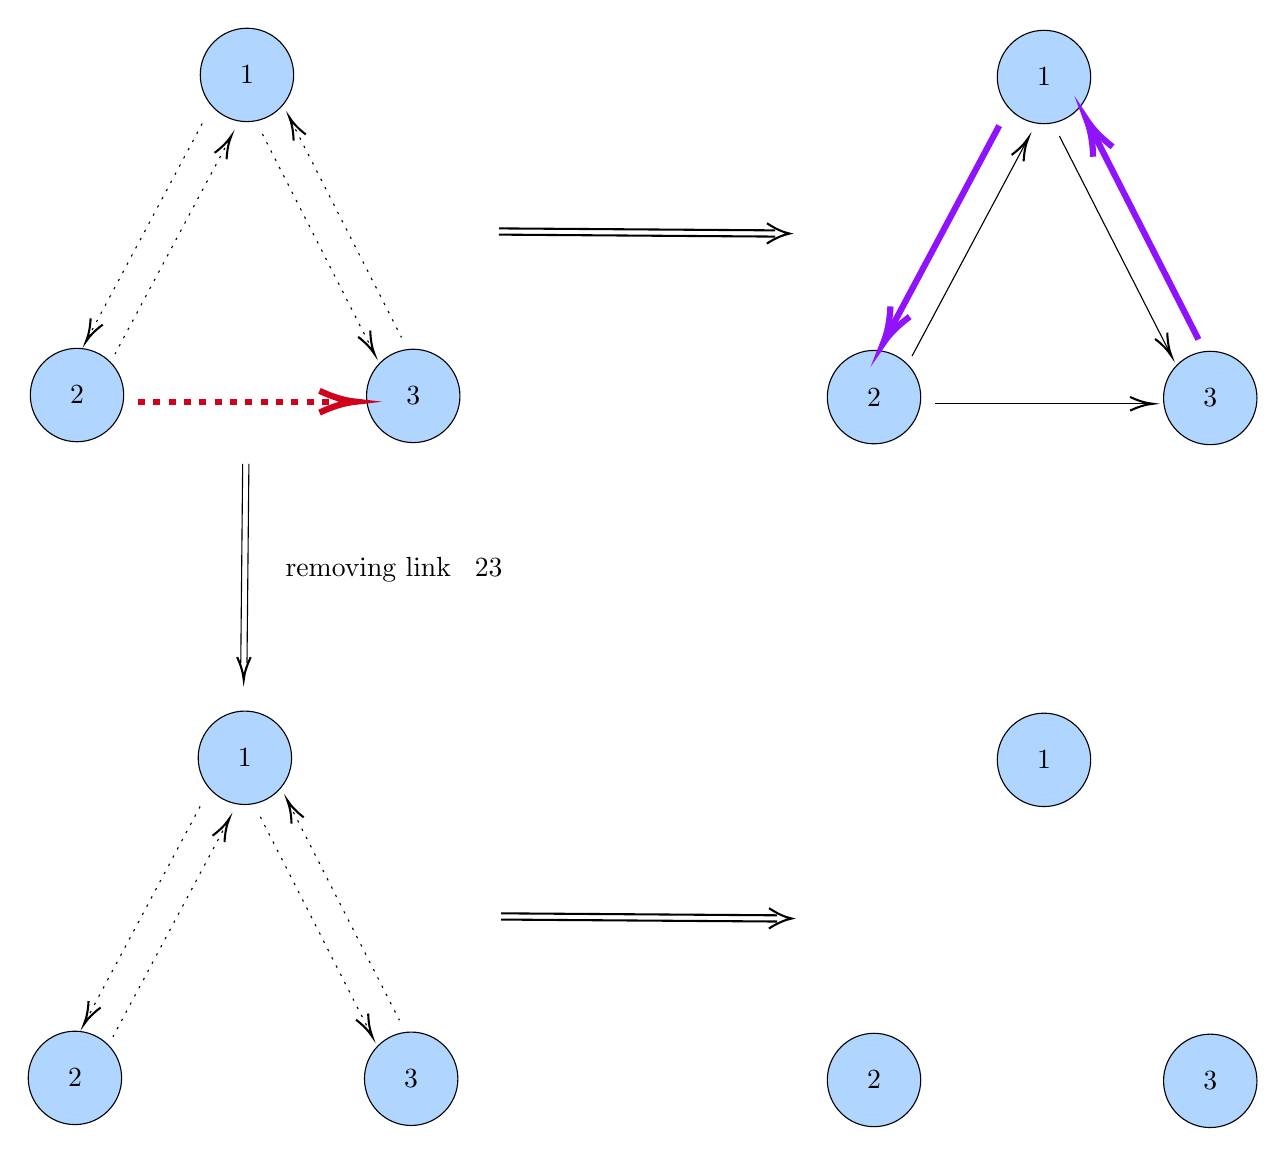
\begin{tikzpicture}[x=0.75pt,y=0.75pt,yscale=-1,xscale=1]
\draw  [fill={rgb, 255:red, 103; green, 174; blue, 255 }  ,fill opacity=0.52 ] (170.07,34.56) .. controls (170.07,22.13) and (180.15,12.06) .. (192.57,12.06) .. controls (205,12.06) and (215.07,22.13) .. (215.07,34.56) .. controls (215.07,46.98) and (205,57.06) .. (192.57,57.06) .. controls (180.15,57.06) and (170.07,46.98) .. (170.07,34.56) -- cycle ;
\draw  [fill={rgb, 255:red, 103; green, 174; blue, 255 }  ,fill opacity=0.52 ] (88.18,188.79) .. controls (88.18,176.36) and (98.25,166.29) .. (110.68,166.29) .. controls (123.1,166.29) and (133.18,176.36) .. (133.18,188.79) .. controls (133.18,201.21) and (123.1,211.29) .. (110.68,211.29) .. controls (98.25,211.29) and (88.18,201.21) .. (88.18,188.79) -- cycle ;
\draw  [fill={rgb, 255:red, 103; green, 174; blue, 255 }  ,fill opacity=0.52 ] (250.18,189.21) .. controls (250.18,176.79) and (260.25,166.71) .. (272.68,166.71) .. controls (285.1,166.71) and (295.18,176.79) .. (295.18,189.21) .. controls (295.18,201.64) and (285.1,211.71) .. (272.68,211.71) .. controls (260.25,211.71) and (250.18,201.64) .. (250.18,189.21) -- cycle ;
\draw  [dash pattern={on 0.84pt off 2.51pt}]  (171,58) -- (115.94,161.24) ;
\draw [shift={(115,163)}, rotate = 298.07] [color={rgb, 255:red, 0; green, 0; blue, 0 }  ][line width=0.75]    (10.93,-3.29) .. controls (6.95,-1.4) and (3.31,-0.3) .. (0,0) .. controls (3.31,0.3) and (6.95,1.4) .. (10.93,3.29)   ;
\draw  [dash pattern={on 0.84pt off 2.51pt}]  (184.06,65.76) -- (129,169) ;
\draw [shift={(185,64)}, rotate = 118.07] [color={rgb, 255:red, 0; green, 0; blue, 0 }  ][line width=0.75]    (10.93,-3.29) .. controls (6.95,-1.4) and (3.31,-0.3) .. (0,0) .. controls (3.31,0.3) and (6.95,1.4) .. (10.93,3.29)   ;
\draw  [dash pattern={on 0.84pt off 2.51pt}]  (200,63) -- (253.09,167.22) ;
\draw [shift={(254,169)}, rotate = 243] [color={rgb, 255:red, 0; green, 0; blue, 0 }  ][line width=0.75]    (10.93,-3.29) .. controls (6.95,-1.4) and (3.31,-0.3) .. (0,0) .. controls (3.31,0.3) and (6.95,1.4) .. (10.93,3.29)   ;
\draw  [dash pattern={on 0.84pt off 2.51pt}]  (213.91,56.78) -- (267,161) ;
\draw [shift={(213,55)}, rotate = 63] [color={rgb, 255:red, 0; green, 0; blue, 0 }  ][line width=0.75]    (10.93,-3.29) .. controls (6.95,-1.4) and (3.31,-0.3) .. (0,0) .. controls (3.31,0.3) and (6.95,1.4) .. (10.93,3.29)   ;
\draw [color={rgb, 255:red, 208; green, 2; blue, 27 }  ,draw opacity=1 ][line width=2.25]  [dash pattern={on 2.53pt off 3.02pt}]  (140,192) -- (241,192) ;
\draw [shift={(245,192)}, rotate = 180] [color={rgb, 255:red, 208; green, 2; blue, 27 }  ,draw opacity=1 ][line width=2.25]    (17.49,-5.26) .. controls (11.12,-2.23) and (5.29,-0.48) .. (0,0) .. controls (5.29,0.48) and (11.12,2.23) .. (17.49,5.26)   ;
\draw  [fill={rgb, 255:red, 103; green, 174; blue, 255 }  ,fill opacity=0.52 ] (169.07,363.56) .. controls (169.07,351.13) and (179.15,341.06) .. (191.57,341.06) .. controls (204,341.06) and (214.07,351.13) .. (214.07,363.56) .. controls (214.07,375.98) and (204,386.06) .. (191.57,386.06) .. controls (179.15,386.06) and (169.07,375.98) .. (169.07,363.56) -- cycle ;
\draw  [fill={rgb, 255:red, 103; green, 174; blue, 255 }  ,fill opacity=0.52 ] (87.18,517.79) .. controls (87.18,505.36) and (97.25,495.29) .. (109.68,495.29) .. controls (122.1,495.29) and (132.18,505.36) .. (132.18,517.79) .. controls (132.18,530.21) and (122.1,540.29) .. (109.68,540.29) .. controls (97.25,540.29) and (87.18,530.21) .. (87.18,517.79) -- cycle ;
\draw  [fill={rgb, 255:red, 103; green, 174; blue, 255 }  ,fill opacity=0.52 ] (249.18,518.21) .. controls (249.18,505.79) and (259.25,495.71) .. (271.68,495.71) .. controls (284.1,495.71) and (294.18,505.79) .. (294.18,518.21) .. controls (294.18,530.64) and (284.1,540.71) .. (271.68,540.71) .. controls (259.25,540.71) and (249.18,530.64) .. (249.18,518.21) -- cycle ;
\draw  [dash pattern={on 0.84pt off 2.51pt}]  (170,387) -- (114.94,490.24) ;
\draw [shift={(114,492)}, rotate = 298.07] [color={rgb, 255:red, 0; green, 0; blue, 0 }  ][line width=0.75]    (10.93,-3.29) .. controls (6.95,-1.4) and (3.31,-0.3) .. (0,0) .. controls (3.31,0.3) and (6.95,1.4) .. (10.93,3.29)   ;
\draw  [dash pattern={on 0.84pt off 2.51pt}]  (183.06,394.76) -- (128,498) ;
\draw [shift={(184,393)}, rotate = 118.07] [color={rgb, 255:red, 0; green, 0; blue, 0 }  ][line width=0.75]    (10.93,-3.29) .. controls (6.95,-1.4) and (3.31,-0.3) .. (0,0) .. controls (3.31,0.3) and (6.95,1.4) .. (10.93,3.29)   ;
\draw  [dash pattern={on 0.84pt off 2.51pt}]  (199,392) -- (252.09,496.22) ;
\draw [shift={(253,498)}, rotate = 243] [color={rgb, 255:red, 0; green, 0; blue, 0 }  ][line width=0.75]    (10.93,-3.29) .. controls (6.95,-1.4) and (3.31,-0.3) .. (0,0) .. controls (3.31,0.3) and (6.95,1.4) .. (10.93,3.29)   ;
\draw  [dash pattern={on 0.84pt off 2.51pt}]  (212.91,385.78) -- (266,490) ;
\draw [shift={(212,384)}, rotate = 63] [color={rgb, 255:red, 0; green, 0; blue, 0 }  ][line width=0.75]    (10.93,-3.29) .. controls (6.95,-1.4) and (3.31,-0.3) .. (0,0) .. controls (3.31,0.3) and (6.95,1.4) .. (10.93,3.29)   ;
\draw  [fill={rgb, 255:red, 103; green, 174; blue, 255 }  ,fill opacity=0.52 ] (554.07,35.56) .. controls (554.07,23.13) and (564.15,13.06) .. (576.57,13.06) .. controls (589,13.06) and (599.07,23.13) .. (599.07,35.56) .. controls (599.07,47.98) and (589,58.06) .. (576.57,58.06) .. controls (564.15,58.06) and (554.07,47.98) .. (554.07,35.56) -- cycle ;
\draw  [fill={rgb, 255:red, 103; green, 174; blue, 255 }  ,fill opacity=0.52 ] (472.18,189.79) .. controls (472.18,177.36) and (482.25,167.29) .. (494.68,167.29) .. controls (507.1,167.29) and (517.18,177.36) .. (517.18,189.79) .. controls (517.18,202.21) and (507.1,212.29) .. (494.68,212.29) .. controls (482.25,212.29) and (472.18,202.21) .. (472.18,189.79) -- cycle ;
\draw  [fill={rgb, 255:red, 103; green, 174; blue, 255 }  ,fill opacity=0.52 ] (634.18,190.21) .. controls (634.18,177.79) and (644.25,167.71) .. (656.68,167.71) .. controls (669.1,167.71) and (679.18,177.79) .. (679.18,190.21) .. controls (679.18,202.64) and (669.1,212.71) .. (656.68,212.71) .. controls (644.25,212.71) and (634.18,202.64) .. (634.18,190.21) -- cycle ;
\draw [color={rgb, 255:red, 144; green, 19; blue, 254 }  ,draw opacity=1 ][line width=2.25]    (555,59) -- (500.88,160.47) ;
\draw [shift={(499,164)}, rotate = 298.07] [color={rgb, 255:red, 144; green, 19; blue, 254 }  ,draw opacity=1 ][line width=2.25]    (17.49,-5.26) .. controls (11.12,-2.23) and (5.29,-0.48) .. (0,0) .. controls (5.29,0.48) and (11.12,2.23) .. (17.49,5.26)   ;
\draw    (568.06,66.76) -- (513,170) ;
\draw [shift={(569,65)}, rotate = 118.07] [color={rgb, 255:red, 0; green, 0; blue, 0 }  ][line width=0.75]    (10.93,-3.29) .. controls (6.95,-1.4) and (3.31,-0.3) .. (0,0) .. controls (3.31,0.3) and (6.95,1.4) .. (10.93,3.29)   ;
\draw    (584,64) -- (637.09,168.22) ;
\draw [shift={(638,170)}, rotate = 243] [color={rgb, 255:red, 0; green, 0; blue, 0 }  ][line width=0.75]    (10.93,-3.29) .. controls (6.95,-1.4) and (3.31,-0.3) .. (0,0) .. controls (3.31,0.3) and (6.95,1.4) .. (10.93,3.29)   ;
\draw [color={rgb, 255:red, 144; green, 19; blue, 254 }  ,draw opacity=1 ][line width=2.25]    (598.82,59.56) -- (651,162) ;
\draw [shift={(597,56)}, rotate = 63] [color={rgb, 255:red, 144; green, 19; blue, 254 }  ,draw opacity=1 ][line width=2.25]    (17.49,-5.26) .. controls (11.12,-2.23) and (5.29,-0.48) .. (0,0) .. controls (5.29,0.48) and (11.12,2.23) .. (17.49,5.26)   ;
\draw    (524,193) -- (627,193) ;
\draw [shift={(629,193)}, rotate = 180] [color={rgb, 255:red, 0; green, 0; blue, 0 }  ][line width=0.75]    (10.93,-3.29) .. controls (6.95,-1.4) and (3.31,-0.3) .. (0,0) .. controls (3.31,0.3) and (6.95,1.4) .. (10.93,3.29)   ;
\draw [line width=0.75]    (314.01,108.5) -- (447.01,109.45)(313.99,111.5) -- (446.99,112.45) ;
\draw [shift={(454,111)}, rotate = 180.41] [color={rgb, 255:red, 0; green, 0; blue, 0 }  ][line width=0.75]    (10.93,-4.9) .. controls (6.95,-2.3) and (3.31,-0.67) .. (0,0) .. controls (3.31,0.67) and (6.95,2.3) .. (10.93,4.9)   ;
\draw  [fill={rgb, 255:red, 103; green, 174; blue, 255 }  ,fill opacity=0.52 ] (554.07,364.56) .. controls (554.07,352.13) and (564.15,342.06) .. (576.57,342.06) .. controls (589,342.06) and (599.07,352.13) .. (599.07,364.56) .. controls (599.07,376.98) and (589,387.06) .. (576.57,387.06) .. controls (564.15,387.06) and (554.07,376.98) .. (554.07,364.56) -- cycle ;
\draw  [fill={rgb, 255:red, 103; green, 174; blue, 255 }  ,fill opacity=0.52 ] (472.18,518.79) .. controls (472.18,506.36) and (482.25,496.29) .. (494.68,496.29) .. controls (507.1,496.29) and (517.18,506.36) .. (517.18,518.79) .. controls (517.18,531.21) and (507.1,541.29) .. (494.68,541.29) .. controls (482.25,541.29) and (472.18,531.21) .. (472.18,518.79) -- cycle ;
\draw  [fill={rgb, 255:red, 103; green, 174; blue, 255 }  ,fill opacity=0.52 ] (634.18,519.21) .. controls (634.18,506.79) and (644.25,496.71) .. (656.68,496.71) .. controls (669.1,496.71) and (679.18,506.79) .. (679.18,519.21) .. controls (679.18,531.64) and (669.1,541.71) .. (656.68,541.71) .. controls (644.25,541.71) and (634.18,531.64) .. (634.18,519.21) -- cycle ;
\draw [line width=0.75]    (315.01,438.5) -- (448.01,439.45)(314.99,441.5) -- (447.99,442.45) ;
\draw [shift={(455,441)}, rotate = 180.41] [color={rgb, 255:red, 0; green, 0; blue, 0 }  ][line width=0.75]    (10.93,-4.9) .. controls (6.95,-2.3) and (3.31,-0.67) .. (0,0) .. controls (3.31,0.67) and (6.95,2.3) .. (10.93,4.9)   ;
\draw    (193.5,222.01) -- (192.58,318.01)(190.5,221.99) -- (189.58,317.99) ;
\draw [shift={(191,326)}, rotate = 270.55] [color={rgb, 255:red, 0; green, 0; blue, 0 }  ][line width=0.75]    (10.93,-3.29) .. controls (6.95,-1.4) and (3.31,-0.3) .. (0,0) .. controls (3.31,0.3) and (6.95,1.4) .. (10.93,3.29)   ;
\draw (192.57,34.56) node    {$1$};
\draw (110.68,188.79) node    {$2$};
\draw (272.68,189.21) node    {$3$};
\draw (271.68,518.21) node    {$3$};
\draw (109.68,517.79) node    {$2$};
\draw (191.57,363.56) node    {$1$};
\draw (656.68,190.21) node    {$3$};
\draw (494.68,189.79) node    {$2$};
\draw (576.57,35.56) node    {$1$};
\draw (656.68,519.21) node    {$3$};
\draw (494.68,518.79) node    {$2$};
\draw (576.57,364.56) node    {$1$};
\draw (251,273) node   [align=left] {removing link};
\draw (309,272) node    {$23$};
\end{tikzpicture}}
\caption{Key removing link in endogenous and exogenous network in Example 4} \label{fig:ex4}
\end{figure}

Next, we introduce key adding link in endogenous and exogenous network similarly.
Key adding link is defined as the link which, once added to the network, generates the highest possible increment in aggreate effort level.

\begin{definition}
	Link $ij$ is {\it{key adding link in endogenous network}} if, given potential network $g^p$,
    \[ ij \in \arg \max_{ij \notin E(g^p)} \{ x^*(g^{**}(\bm{\psi}({g^p}^{+ij}, \bm{C}))) - x^*(g^{**}(\bm{\psi}(g^p, \bm{C}))) \} \]
    where ${g^p}^{+ij}$ is network obtained by adding link $ij$ to $g^p$
\end{definition}

\begin{definition}
	Link $ij$ is {\it{key adding link in exogenous network}} if, given network $g$,
    \[ ij \in \arg \max_{ij \notin E(g)} \{ x^*(g^{+ij}) - x^*(g) \} \]
    where $g^{+ij}$ is network obtained by adding link $ij$ to $g$
\end{definition}

In the context of web advertisement network, key adding link is the advertisement on the page which brings the highest increment in aggregate effort level.
For a policy maker, key adding link is the connection which he should recommend the web page owner to make.
By encouraging to connect and putting the advertisement, a policy maker can raise the level of investment on the web page.
Following example shows key adding link in endogenous and exogenous network might be different.

\begin{example}
Suppose $n=3$, $\bm{\alpha} = (1,1,1)$ and $\phi = 1/3$.
Consider potential network $g^p$ and link formation costs are
\[
\bm{G}^p = \left[
            \begin{array}{ccc}
                0 & 1 & 1 \\
                1 & 0 & 0 \\
                1 & 0 & 0
            \end{array} \right]
\text{and} \ 
\bm{C} = \left[
                \begin{array}{ccc}
                    0 & 0.1 & 0.1 \\
                    1 & 0 & 0 \\
                    1 & 0 & 0
                \end{array} \right] \]
Then, the greatest equilibrium network $g^{**}$ becomes
\[ \bm{G}^{**} = \left[
    \begin{array}{ccc}
        0 & 1 & 1 \\
        0 & 0 & 0 \\
        0 & 0 & 0
    \end{array} \right]\]
By considering $g^{**}$ as exogenous network, key adding link in exogenoous network is link $21$ and $31$.
But, in this example, key removing in endogenous network is link $23$ and $32$.
We can increase the aggregate level of efforts by adding link $23$ or link $32$ to the potential network $g^p$.
See Figure \ref{fig:ex5} (red arrow and blue arrow represent key adding link in endogenous and exogenous network respectively).
\end{example}

\begin{figure}[h]
\centering
\tikzset{every picture/.style={line width=0.75pt}}
\scalebox{0.75}[0.75]{
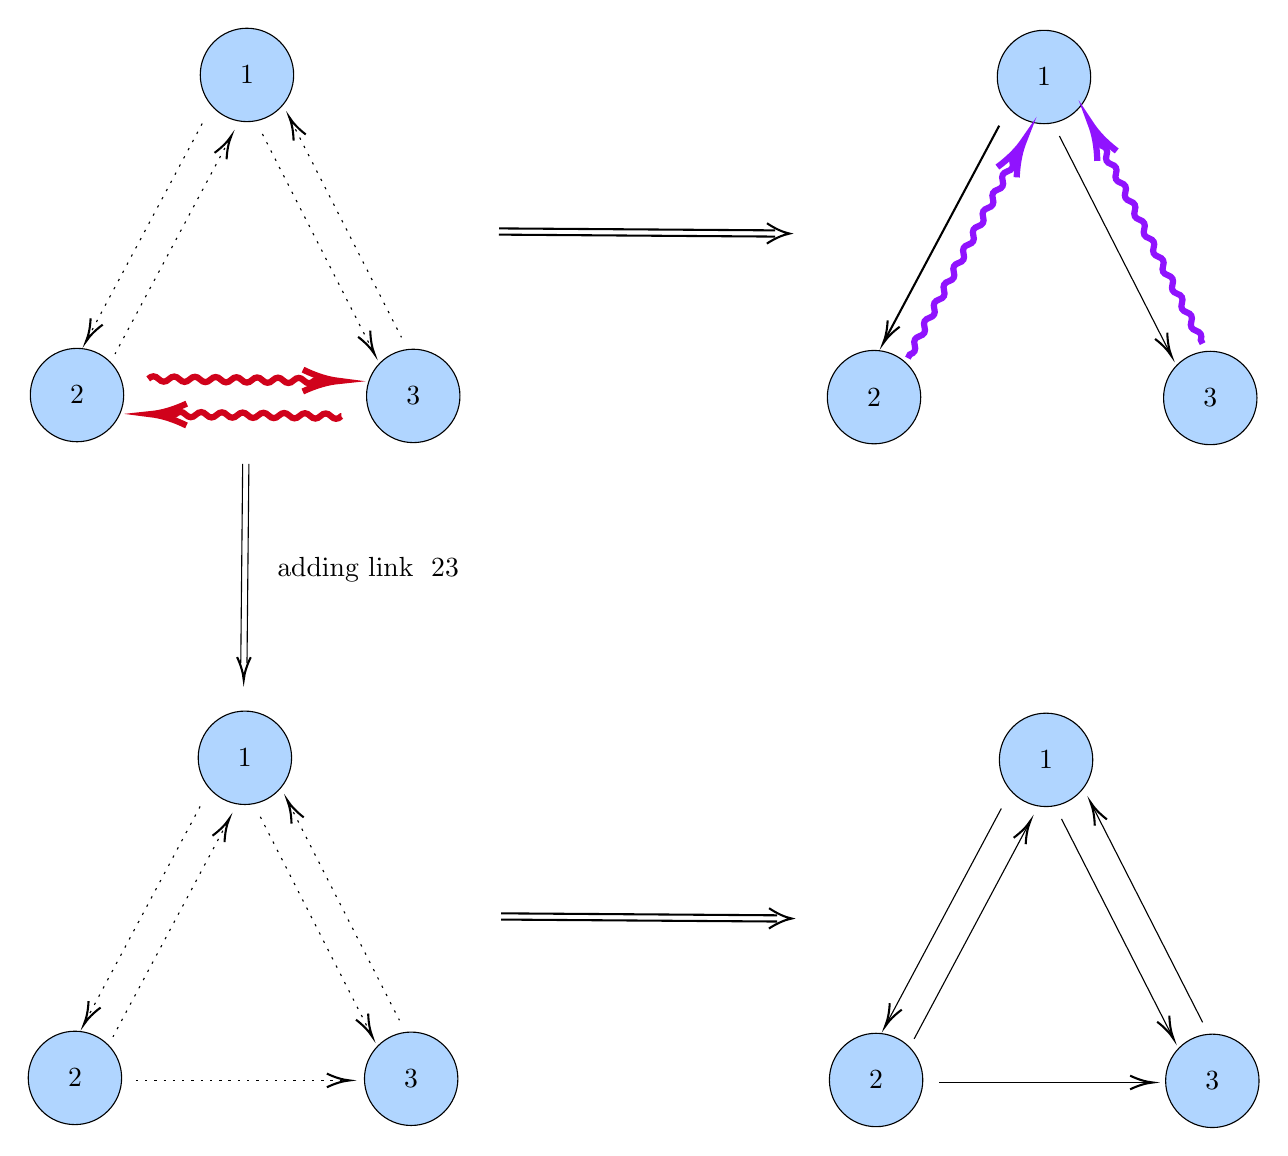
\begin{tikzpicture}[x=0.75pt,y=0.75pt,yscale=-1,xscale=1]
\draw  [fill={rgb, 255:red, 103; green, 174; blue, 255 }  ,fill opacity=0.52 ] (190.07,54.56) .. controls (190.07,42.13) and (200.15,32.06) .. (212.57,32.06) .. controls (225,32.06) and (235.07,42.13) .. (235.07,54.56) .. controls (235.07,66.98) and (225,77.06) .. (212.57,77.06) .. controls (200.15,77.06) and (190.07,66.98) .. (190.07,54.56) -- cycle ;
\draw  [fill={rgb, 255:red, 103; green, 174; blue, 255 }  ,fill opacity=0.52 ] (108.18,208.79) .. controls (108.18,196.36) and (118.25,186.29) .. (130.68,186.29) .. controls (143.1,186.29) and (153.18,196.36) .. (153.18,208.79) .. controls (153.18,221.21) and (143.1,231.29) .. (130.68,231.29) .. controls (118.25,231.29) and (108.18,221.21) .. (108.18,208.79) -- cycle ;
\draw  [fill={rgb, 255:red, 103; green, 174; blue, 255 }  ,fill opacity=0.52 ] (270.18,209.21) .. controls (270.18,196.79) and (280.25,186.71) .. (292.68,186.71) .. controls (305.1,186.71) and (315.18,196.79) .. (315.18,209.21) .. controls (315.18,221.64) and (305.1,231.71) .. (292.68,231.71) .. controls (280.25,231.71) and (270.18,221.64) .. (270.18,209.21) -- cycle ;
\draw  [dash pattern={on 0.84pt off 2.51pt}]  (191,78) -- (135.94,181.24) ;
\draw [shift={(135,183)}, rotate = 298.07] [color={rgb, 255:red, 0; green, 0; blue, 0 }  ][line width=0.75]    (10.93,-3.29) .. controls (6.95,-1.4) and (3.31,-0.3) .. (0,0) .. controls (3.31,0.3) and (6.95,1.4) .. (10.93,3.29)   ;
\draw  [dash pattern={on 0.84pt off 2.51pt}]  (204.06,85.76) -- (149,189) ;
\draw [shift={(205,84)}, rotate = 118.07] [color={rgb, 255:red, 0; green, 0; blue, 0 }  ][line width=0.75]    (10.93,-3.29) .. controls (6.95,-1.4) and (3.31,-0.3) .. (0,0) .. controls (3.31,0.3) and (6.95,1.4) .. (10.93,3.29)   ;
\draw  [dash pattern={on 0.84pt off 2.51pt}]  (220,83) -- (273.09,187.22) ;
\draw [shift={(274,189)}, rotate = 243] [color={rgb, 255:red, 0; green, 0; blue, 0 }  ][line width=0.75]    (10.93,-3.29) .. controls (6.95,-1.4) and (3.31,-0.3) .. (0,0) .. controls (3.31,0.3) and (6.95,1.4) .. (10.93,3.29)   ;
\draw  [dash pattern={on 0.84pt off 2.51pt}]  (233.91,76.78) -- (287,181) ;
\draw [shift={(233,75)}, rotate = 63] [color={rgb, 255:red, 0; green, 0; blue, 0 }  ][line width=0.75]    (10.93,-3.29) .. controls (6.95,-1.4) and (3.31,-0.3) .. (0,0) .. controls (3.31,0.3) and (6.95,1.4) .. (10.93,3.29)   ;
\draw  [fill={rgb, 255:red, 103; green, 174; blue, 255 }  ,fill opacity=0.52 ] (189.07,383.56) .. controls (189.07,371.13) and (199.15,361.06) .. (211.57,361.06) .. controls (224,361.06) and (234.07,371.13) .. (234.07,383.56) .. controls (234.07,395.98) and (224,406.06) .. (211.57,406.06) .. controls (199.15,406.06) and (189.07,395.98) .. (189.07,383.56) -- cycle ;
\draw  [fill={rgb, 255:red, 103; green, 174; blue, 255 }  ,fill opacity=0.52 ] (107.18,537.79) .. controls (107.18,525.36) and (117.25,515.29) .. (129.68,515.29) .. controls (142.1,515.29) and (152.18,525.36) .. (152.18,537.79) .. controls (152.18,550.21) and (142.1,560.29) .. (129.68,560.29) .. controls (117.25,560.29) and (107.18,550.21) .. (107.18,537.79) -- cycle ;
\draw  [fill={rgb, 255:red, 103; green, 174; blue, 255 }  ,fill opacity=0.52 ] (269.18,538.21) .. controls (269.18,525.79) and (279.25,515.71) .. (291.68,515.71) .. controls (304.1,515.71) and (314.18,525.79) .. (314.18,538.21) .. controls (314.18,550.64) and (304.1,560.71) .. (291.68,560.71) .. controls (279.25,560.71) and (269.18,550.64) .. (269.18,538.21) -- cycle ;
\draw  [dash pattern={on 0.84pt off 2.51pt}]  (190,407) -- (134.94,510.24) ;
\draw [shift={(134,512)}, rotate = 298.07] [color={rgb, 255:red, 0; green, 0; blue, 0 }  ][line width=0.75]    (10.93,-3.29) .. controls (6.95,-1.4) and (3.31,-0.3) .. (0,0) .. controls (3.31,0.3) and (6.95,1.4) .. (10.93,3.29)   ;
\draw  [dash pattern={on 0.84pt off 2.51pt}]  (203.06,414.76) -- (148,518) ;
\draw [shift={(204,413)}, rotate = 118.07] [color={rgb, 255:red, 0; green, 0; blue, 0 }  ][line width=0.75]    (10.93,-3.29) .. controls (6.95,-1.4) and (3.31,-0.3) .. (0,0) .. controls (3.31,0.3) and (6.95,1.4) .. (10.93,3.29)   ;
\draw  [dash pattern={on 0.84pt off 2.51pt}]  (219,412) -- (272.09,516.22) ;
\draw [shift={(273,518)}, rotate = 243] [color={rgb, 255:red, 0; green, 0; blue, 0 }  ][line width=0.75]    (10.93,-3.29) .. controls (6.95,-1.4) and (3.31,-0.3) .. (0,0) .. controls (3.31,0.3) and (6.95,1.4) .. (10.93,3.29)   ;
\draw  [dash pattern={on 0.84pt off 2.51pt}]  (232.91,405.78) -- (286,510) ;
\draw [shift={(232,404)}, rotate = 63] [color={rgb, 255:red, 0; green, 0; blue, 0 }  ][line width=0.75]    (10.93,-3.29) .. controls (6.95,-1.4) and (3.31,-0.3) .. (0,0) .. controls (3.31,0.3) and (6.95,1.4) .. (10.93,3.29)   ;
\draw  [fill={rgb, 255:red, 103; green, 174; blue, 255 }  ,fill opacity=0.52 ] (574.07,55.56) .. controls (574.07,43.13) and (584.15,33.06) .. (596.57,33.06) .. controls (609,33.06) and (619.07,43.13) .. (619.07,55.56) .. controls (619.07,67.98) and (609,78.06) .. (596.57,78.06) .. controls (584.15,78.06) and (574.07,67.98) .. (574.07,55.56) -- cycle ;
\draw  [fill={rgb, 255:red, 103; green, 174; blue, 255 }  ,fill opacity=0.52 ] (492.18,209.79) .. controls (492.18,197.36) and (502.25,187.29) .. (514.68,187.29) .. controls (527.1,187.29) and (537.18,197.36) .. (537.18,209.79) .. controls (537.18,222.21) and (527.1,232.29) .. (514.68,232.29) .. controls (502.25,232.29) and (492.18,222.21) .. (492.18,209.79) -- cycle ;
\draw  [fill={rgb, 255:red, 103; green, 174; blue, 255 }  ,fill opacity=0.52 ] (654.18,210.21) .. controls (654.18,197.79) and (664.25,187.71) .. (676.68,187.71) .. controls (689.1,187.71) and (699.18,197.79) .. (699.18,210.21) .. controls (699.18,222.64) and (689.1,232.71) .. (676.68,232.71) .. controls (664.25,232.71) and (654.18,222.64) .. (654.18,210.21) -- cycle ;
\draw [color={rgb, 255:red, 0; green, 0; blue, 0 }  ,draw opacity=1 ][line width=0.75]    (575,79) -- (519.94,182.24) ;
\draw [shift={(519,184)}, rotate = 298.07] [color={rgb, 255:red, 0; green, 0; blue, 0 }  ,draw opacity=1 ][line width=0.75]    (10.93,-3.29) .. controls (6.95,-1.4) and (3.31,-0.3) .. (0,0) .. controls (3.31,0.3) and (6.95,1.4) .. (10.93,3.29)   ;
\draw    (604,84) -- (657.09,188.22) ;
\draw [shift={(658,190)}, rotate = 243] [color={rgb, 255:red, 0; green, 0; blue, 0 }  ][line width=0.75]    (10.93,-3.29) .. controls (6.95,-1.4) and (3.31,-0.3) .. (0,0) .. controls (3.31,0.3) and (6.95,1.4) .. (10.93,3.29)   ;
\draw [line width=0.75]    (334.01,128.5) -- (467.01,129.45)(333.99,131.5) -- (466.99,132.45) ;
\draw [shift={(474,131)}, rotate = 180.41] [color={rgb, 255:red, 0; green, 0; blue, 0 }  ][line width=0.75]    (10.93,-4.9) .. controls (6.95,-2.3) and (3.31,-0.67) .. (0,0) .. controls (3.31,0.67) and (6.95,2.3) .. (10.93,4.9)   ;
\draw [line width=0.75]    (335.01,458.5) -- (468.01,459.45)(334.99,461.5) -- (467.99,462.45) ;
\draw [shift={(475,461)}, rotate = 180.41] [color={rgb, 255:red, 0; green, 0; blue, 0 }  ][line width=0.75]    (10.93,-4.9) .. controls (6.95,-2.3) and (3.31,-0.67) .. (0,0) .. controls (3.31,0.67) and (6.95,2.3) .. (10.93,4.9)   ;
\draw    (213.5,242.01) -- (212.58,338.01)(210.5,241.99) -- (209.58,337.99) ;
\draw [shift={(211,346)}, rotate = 270.55] [color={rgb, 255:red, 0; green, 0; blue, 0 }  ][line width=0.75]    (10.93,-3.29) .. controls (6.95,-1.4) and (3.31,-0.3) .. (0,0) .. controls (3.31,0.3) and (6.95,1.4) .. (10.93,3.29)   ;
\draw  [dash pattern={on 0.84pt off 2.51pt}]  (159,539) -- (260,539) ;
\draw [shift={(262,539)}, rotate = 180] [color={rgb, 255:red, 0; green, 0; blue, 0 }  ][line width=0.75]    (10.93,-3.29) .. controls (6.95,-1.4) and (3.31,-0.3) .. (0,0) .. controls (3.31,0.3) and (6.95,1.4) .. (10.93,3.29)   ;
\draw  [fill={rgb, 255:red, 103; green, 174; blue, 255 }  ,fill opacity=0.52 ] (575.07,384.56) .. controls (575.07,372.13) and (585.15,362.06) .. (597.57,362.06) .. controls (610,362.06) and (620.07,372.13) .. (620.07,384.56) .. controls (620.07,396.98) and (610,407.06) .. (597.57,407.06) .. controls (585.15,407.06) and (575.07,396.98) .. (575.07,384.56) -- cycle ;
\draw  [fill={rgb, 255:red, 103; green, 174; blue, 255 }  ,fill opacity=0.52 ] (493.18,538.79) .. controls (493.18,526.36) and (503.25,516.29) .. (515.68,516.29) .. controls (528.1,516.29) and (538.18,526.36) .. (538.18,538.79) .. controls (538.18,551.21) and (528.1,561.29) .. (515.68,561.29) .. controls (503.25,561.29) and (493.18,551.21) .. (493.18,538.79) -- cycle ;
\draw  [fill={rgb, 255:red, 103; green, 174; blue, 255 }  ,fill opacity=0.52 ] (655.18,539.21) .. controls (655.18,526.79) and (665.25,516.71) .. (677.68,516.71) .. controls (690.1,516.71) and (700.18,526.79) .. (700.18,539.21) .. controls (700.18,551.64) and (690.1,561.71) .. (677.68,561.71) .. controls (665.25,561.71) and (655.18,551.64) .. (655.18,539.21) -- cycle ;
\draw    (576,408) -- (520.94,511.24) ;
\draw [shift={(520,513)}, rotate = 298.07] [color={rgb, 255:red, 0; green, 0; blue, 0 }  ][line width=0.75]    (10.93,-3.29) .. controls (6.95,-1.4) and (3.31,-0.3) .. (0,0) .. controls (3.31,0.3) and (6.95,1.4) .. (10.93,3.29)   ;
\draw    (589.06,415.76) -- (534,519) ;
\draw [shift={(590,414)}, rotate = 118.07] [color={rgb, 255:red, 0; green, 0; blue, 0 }  ][line width=0.75]    (10.93,-3.29) .. controls (6.95,-1.4) and (3.31,-0.3) .. (0,0) .. controls (3.31,0.3) and (6.95,1.4) .. (10.93,3.29)   ;
\draw    (605,413) -- (658.09,517.22) ;
\draw [shift={(659,519)}, rotate = 243] [color={rgb, 255:red, 0; green, 0; blue, 0 }  ][line width=0.75]    (10.93,-3.29) .. controls (6.95,-1.4) and (3.31,-0.3) .. (0,0) .. controls (3.31,0.3) and (6.95,1.4) .. (10.93,3.29)   ;
\draw    (619.91,406.78) -- (673,511) ;
\draw [shift={(619,405)}, rotate = 63] [color={rgb, 255:red, 0; green, 0; blue, 0 }  ][line width=0.75]    (10.93,-3.29) .. controls (6.95,-1.4) and (3.31,-0.3) .. (0,0) .. controls (3.31,0.3) and (6.95,1.4) .. (10.93,3.29)   ;
\draw    (546,540) -- (647,540) ;
\draw [shift={(649,540)}, rotate = 180] [color={rgb, 255:red, 0; green, 0; blue, 0 }  ][line width=0.75]    (10.93,-3.29) .. controls (6.95,-1.4) and (3.31,-0.3) .. (0,0) .. controls (3.31,0.3) and (6.95,1.4) .. (10.93,3.29)   ;
\draw [color={rgb, 255:red, 208; green, 2; blue, 27 }  ,draw opacity=1 ][line width=2.25]    (165,201) .. controls (166.68,199.35) and (168.35,199.37) .. (170,201.05) .. controls (171.65,202.74) and (173.31,202.76) .. (175,201.11) .. controls (176.68,199.46) and (178.35,199.48) .. (180,201.16) .. controls (181.65,202.85) and (183.31,202.87) .. (185,201.22) .. controls (186.68,199.57) and (188.35,199.59) .. (190,201.27) .. controls (191.65,202.96) and (193.31,202.98) .. (195,201.33) .. controls (196.68,199.68) and (198.35,199.7) .. (200,201.38) .. controls (201.65,203.06) and (203.32,203.08) .. (205,201.43) .. controls (206.69,199.78) and (208.35,199.8) .. (210,201.49) .. controls (211.65,203.17) and (213.32,203.19) .. (215,201.54) .. controls (216.69,199.89) and (218.35,199.91) .. (220,201.6) .. controls (221.65,203.28) and (223.32,203.3) .. (225,201.65) .. controls (226.69,200) and (228.35,200.02) .. (230,201.71) .. controls (231.65,203.39) and (233.32,203.41) .. (235,201.76) .. controls (236.69,200.11) and (238.35,200.13) .. (240,201.82) .. controls (241.65,203.5) and (243.32,203.52) .. (245,201.87) -- (245,201.87) -- (253,201.96) ;
\draw [shift={(257,202)}, rotate = 180.62] [color={rgb, 255:red, 208; green, 2; blue, 27 }  ,draw opacity=1 ][line width=2.25]    (17.49,-5.26) .. controls (11.12,-2.23) and (5.29,-0.48) .. (0,0) .. controls (5.29,0.48) and (11.12,2.23) .. (17.49,5.26)   ;
\draw [color={rgb, 255:red, 208; green, 2; blue, 27 }  ,draw opacity=1 ][line width=2.25]    (170,218.04) -- (178,218.13) .. controls (179.68,216.48) and (181.35,216.5) .. (183,218.18) .. controls (184.65,219.87) and (186.31,219.89) .. (188,218.24) .. controls (189.68,216.59) and (191.35,216.61) .. (193,218.29) .. controls (194.65,219.98) and (196.31,220) .. (198,218.35) .. controls (199.68,216.7) and (201.35,216.72) .. (203,218.4) .. controls (204.65,220.09) and (206.31,220.11) .. (208,218.46) .. controls (209.68,216.81) and (211.35,216.83) .. (213,218.51) .. controls (214.65,220.2) and (216.31,220.22) .. (218,218.57) .. controls (219.68,216.92) and (221.35,216.94) .. (223,218.62) .. controls (224.65,220.3) and (226.32,220.32) .. (228,218.67) .. controls (229.69,217.02) and (231.35,217.04) .. (233,218.73) .. controls (234.65,220.41) and (236.32,220.43) .. (238,218.78) .. controls (239.69,217.13) and (241.35,217.15) .. (243,218.84) .. controls (244.65,220.52) and (246.32,220.54) .. (248,218.89) .. controls (249.69,217.24) and (251.35,217.26) .. (252.99,218.95) .. controls (254.64,220.63) and (256.31,220.65) .. (257.99,219) -- (258,219) -- (258,219) ;
\draw [shift={(166,218)}, rotate = 0.62] [color={rgb, 255:red, 208; green, 2; blue, 27 }  ,draw opacity=1 ][line width=2.25]    (17.49,-5.26) .. controls (11.12,-2.23) and (5.29,-0.48) .. (0,0) .. controls (5.29,0.48) and (11.12,2.23) .. (17.49,5.26)   ;
\draw [color={rgb, 255:red, 144; green, 19; blue, 254 }  ,draw opacity=1 ][line width=2.25]    (585.12,89.53) -- (581.35,96.59) .. controls (582.04,98.84) and (581.25,100.31) .. (579,101) .. controls (576.75,101.69) and (575.96,103.16) .. (576.65,105.41) .. controls (577.33,107.66) and (576.54,109.13) .. (574.29,109.82) .. controls (572.04,110.51) and (571.25,111.99) .. (571.94,114.24) .. controls (572.63,116.49) and (571.84,117.96) .. (569.59,118.65) .. controls (567.34,119.34) and (566.55,120.81) .. (567.24,123.06) .. controls (567.92,125.31) and (567.13,126.78) .. (564.88,127.47) .. controls (562.63,128.16) and (561.84,129.63) .. (562.53,131.88) .. controls (563.22,134.13) and (562.43,135.6) .. (560.18,136.29) .. controls (557.92,136.98) and (557.13,138.45) .. (557.82,140.71) .. controls (558.51,142.96) and (557.72,144.43) .. (555.47,145.12) .. controls (553.22,145.81) and (552.43,147.28) .. (553.12,149.53) .. controls (553.8,151.78) and (553.01,153.25) .. (550.76,153.94) .. controls (548.51,154.63) and (547.72,156.1) .. (548.41,158.35) .. controls (549.1,160.6) and (548.31,162.07) .. (546.06,162.76) .. controls (543.81,163.45) and (543.02,164.93) .. (543.71,167.18) .. controls (544.39,169.43) and (543.6,170.9) .. (541.35,171.59) .. controls (539.1,172.28) and (538.31,173.75) .. (539,176) .. controls (539.69,178.25) and (538.9,179.72) .. (536.65,180.41) .. controls (534.4,181.1) and (533.61,182.57) .. (534.29,184.82) .. controls (534.98,187.07) and (534.19,188.55) .. (531.94,189.24) -- (531,191) -- (531,191) ;
\draw [shift={(587,86)}, rotate = 118.07] [color={rgb, 255:red, 144; green, 19; blue, 254 }  ,draw opacity=1 ][line width=2.25]    (17.49,-5.26) .. controls (11.12,-2.23) and (5.29,-0.48) .. (0,0) .. controls (5.29,0.48) and (11.12,2.23) .. (17.49,5.26)   ;
\draw [color={rgb, 255:red, 144; green, 19; blue, 254 }  ,draw opacity=1 ][line width=2.25]    (620.82,81.56) -- (624.45,88.69) .. controls (626.69,89.42) and (627.45,90.91) .. (626.72,93.15) .. controls (625.99,95.39) and (626.75,96.87) .. (628.99,97.6) .. controls (631.23,98.33) and (631.99,99.82) .. (631.26,102.06) .. controls (630.53,104.3) and (631.29,105.78) .. (633.53,106.51) .. controls (635.77,107.24) and (636.53,108.73) .. (635.8,110.97) .. controls (635.07,113.21) and (635.82,114.69) .. (638.06,115.42) .. controls (640.3,116.15) and (641.06,117.64) .. (640.33,119.88) .. controls (639.6,122.12) and (640.36,123.6) .. (642.6,124.33) .. controls (644.84,125.06) and (645.6,126.55) .. (644.87,128.79) .. controls (644.14,131.03) and (644.9,132.51) .. (647.14,133.24) .. controls (649.38,133.97) and (650.14,135.46) .. (649.41,137.7) .. controls (648.68,139.94) and (649.44,141.42) .. (651.68,142.15) .. controls (653.92,142.88) and (654.68,144.37) .. (653.95,146.61) .. controls (653.22,148.85) and (653.98,150.34) .. (656.22,151.07) .. controls (658.46,151.8) and (659.22,153.28) .. (658.49,155.52) .. controls (657.76,157.76) and (658.52,159.25) .. (660.76,159.98) .. controls (663,160.71) and (663.76,162.19) .. (663.03,164.43) .. controls (662.3,166.67) and (663.06,168.16) .. (665.3,168.89) .. controls (667.54,169.62) and (668.3,171.1) .. (667.57,173.34) .. controls (666.84,175.58) and (667.6,177.07) .. (669.84,177.8) .. controls (672.08,178.53) and (672.84,180.01) .. (672.11,182.25) -- (673,184) -- (673,184) ;
\draw [shift={(619,78)}, rotate = 63] [color={rgb, 255:red, 144; green, 19; blue, 254 }  ,draw opacity=1 ][line width=2.25]    (17.49,-5.26) .. controls (11.12,-2.23) and (5.29,-0.48) .. (0,0) .. controls (5.29,0.48) and (11.12,2.23) .. (17.49,5.26)   ;
\draw (260,293) node   [align=left] {adding link};
\draw (308,292) node    {$23$};
\draw (676.68,210.21) node    {$3$};
\draw (514.68,209.79) node    {$2$};
\draw (596.57,55.56) node    {$1$};
\draw (291.68,538.21) node    {$3$};
\draw (129.68,537.79) node    {$2$};
\draw (211.57,383.56) node    {$1$};
\draw (292.68,209.21) node    {$3$};
\draw (130.68,208.79) node    {$2$};
\draw (212.57,54.56) node    {$1$};
\draw (677.68,539.21) node    {$3$};
\draw (515.68,538.79) node    {$2$};
\draw (597.57,384.56) node    {$1$};
\end{tikzpicture}}
\caption{Key adding link in endogenous and exogenous network} \label{fig:ex5}
\end{figure}

From all thse example, we can see that key link policy can be different between endogenous and exogenous network.
Therefore, we have to incorporate the endogeneity of the network to consider the policy implications.
Again, due to the complexity of the relationship between link formation costs and realized network, we cannot propose the proposition who is the key player in endogenous network.
The closed form solution to identify the key player is remaining for future work.


\section{Conclusion}

This paper argues the game with externality in the endogenously formed network.
Contrary to the previous literatures, agents endogenously form the network.
In the model, agents choose their neighbors in the potential network at first, and then the network is realized.
When agents form links to neighbors, they incur the link-specific costs and these costs play an important role in the agents' decisions and the formation of network.
Next, agents decide their effort level in this formed network, and their decisions generates the externality, peer effect, through the network.
We focus on the subgame perfect equilibrium where agents take pure strategies in each stage.
We show that there always exists the equilibrium for any potential network and link formation costs.
Behind this result, there are supermodurality in the 1st stage game given 2nd stage equilibrium.
However, the realized network high dimensional discontiunous function in the costs, so it is difficult to identify the structure of the network from the link formation costs.
We can find the key player in the endogenous network is not necessarily same with the one in the exogenous network, which implies that we might have a wrong policy implication.
Therefore, it is significant to consider the mechanism of network formation.

Some weaknesses in our model are remaining for the future work.
First, link formation is accomplished by the unilateral decisions.
This is mainly due to the simplification of the analysis.
In reality, the relationships are made by the bilateral agreement, such as friendship network and firm-to-firm relationship.
In such a model, the network is treated as undirected network.
To incorporate the bilateral decisions, in the model similar to ours, we have to consider the complex belief system: when I offer the relationship, will she accept my offer?
The beliefs depend on other agents' decisions and beliefs, so it is not easy to bilateral link formation.
Second, links don't have any weights, unweighted network.
In many situations, relationships have unequal importances, for example, the closeness of friends are not equal in the social network.
In order to make the links weighted, agents have to deecide the link weights when they form relationships.
Our model can be extened to the unweighted network when agents choose the intensity of each forming links like Kim, J., Patacchini, E., Picard, P.M. and Y. Zenou (2017)~\cite{Urban}.
However, in such a model, agents form links to all other agents (weights are unequal), that is, realized network becomes complete network.
This is not appropriate for representing the real environment.
Finally, our model should be extended to various kinds of utility forms.
Currently, we can only explore the model with positive peer effects in the network, but these are many networks such that the externalities does not exist or are not appropriate to apply.
For example, our model is not suitable for analyzing the production network because we cannot incorporate the price of goods or production functions and the peer effect is not significant.
The analizing mechanism of network formation is important for policy implication.
It enables us to analyze the effect of intervention to the network on the allocation of goods or the social welfare.
Analyzing various kinds of network formation opens the way to "network design" field.

\appendix

\section{Appendix}

\begin{proof}[Proof of Proposition 1.]
	For all pair $ij$, from the definition of $g$ and $g^p$, $g_{ij} \ge 0$, $g_{ij}^p \ge 0$, and $g_{ij}^p \ge g_{ij}$.
	By the theorem $\text{I}^*$ of Debreu and Herstein (1952)~\cite{debreu}, we can have
	\[ \rho(\bm{G}^p) \ge \rho(\bm{G})  \]
	Since $\phi > 0$, by Assumption 1, $\phi \rho(\bm{G}) < 1$.
	By Theorem 1 of Ballester, Calv\'{o}-Armengol and Zenou (2005)~\cite{whowho}, we can have a unique Nash equilibrium $\bm{x}^*$, which is interior and given by
	\[ \bm{x}^* = {(\bm{I} - \phi \bm{G})}^{-1} \bm{\alpha} \] 
\end{proof}

\begin{proof}[Proof of Lemma 1.]
	We can write
	\[ \bm{x}(g) = {(\bm{I} - \phi \bm{G})}^{-1} \bm{\alpha} = \sum_{p=0}^{\infty} \phi^p \bm{G}^p \bm{\alpha} \]
	\[ \bm{x}(\hat{g}) = {(\bm{I} - \phi \bm{\hat{G}})}^{-1} \bm{\alpha} = \sum_{p=0}^{\infty} \phi^p \bm{\hat{G}}^p \bm{\alpha} \]
	Therefore,
	\begin{eqnarray}
		\label{lemma1-1}
		\bm{x}^*(\hat{g}) - \bm{x}^*(g) &=& \sum_{p=0}^{\infty} \phi^p \bm{\hat{G}}^p \bm{\alpha} - \sum_{p=0}^{\infty} \phi^p \bm{G}^p \bm{\alpha} \notag \\
										&=& \sum_{p=0}^{\infty} \phi^p (\bm{\hat{G}}^p - \bm{G}^p) \bm{\alpha} \notag \\
										&=& \phi (\bm{\hat{G}} - \bm{G}) \bm{\alpha} + \phi^2 (\bm{\hat{G}}^2 - \bm{G}^2) \bm{\alpha} + \cdots
	\end{eqnarray}
	By construction, we can write $\bm{\hat{G}} = \bm{G} + \bm{D}$ where $d_{ij} \in \{0,1\}$.
	Then, the right hand side of (\ref{lemma1-1}) can be written as
	\[ \phi \bm{D} \bm{\alpha} + \phi (\bm{G} \bm{D} + \bm{D} \bm{G} + \bm{D}^2) \bm{\alpha} + \cdots \]
	Since $\bm{G}$ and $\bm{D}$ are both nonnegative matrices, their combinations are also nonnegative.
	Therefore, we have
	\begin{eqnarray*}
		\phi \bm{D} \bm{\alpha} + \phi (\bm{G} \bm{D} + \bm{D} \bm{G} + \bm{D}^2) \bm{\alpha} + \cdots &\ge& \bm{0} \\
		\Leftrightarrow \bm{x}^*(\hat{g}) - \bm{x}^*(g) &\ge& \bm{0}
	\end{eqnarray*}
	In addition, since, for some $j$, $\hat{g}_{ij} - g_{ij} = 1$, $\alpha_j > 0$, and $\phi > 0$, $i$-th element of $\phi \bm{D} \bm{\alpha}$ is strictly greater than $0$.
	That is, $i$-th element of $\bm{x}^*(\hat{g}) - \bm{x}^*(g)$ is strictly greater than $0$.
	Thus, we have
	\[ x_i^*(\hat{g}) > x_i^*(g) \]
\end{proof}

\begin{proof}[Proof of Lemma 2.]
	Here, we abbreviate the strategies $\bm{\psi}$.
	Let $\bm{D}$ be the matrix such that $d_{ij} \in \{0,1\}$.
	Then, we can write $\bm{\hat{G}} = \bm{G} + \bm{D}$ and $\bm{\hat{H}} = \bm{H} + \bm{D}$.
	We can have
	\begin{eqnarray*}
		\bm{x}^*(\hat{g}) - \bm{x}^*(g)
			&=& \sum_{p=0}^{\infty} \phi^p \bm{\hat{G}}^p \bm{\alpha} - \sum_{p=0}^{\infty} \phi^p \bm{G}^p \bm{\alpha} \\
			&=& \sum_{p=0}^{\infty} \phi^p (\bm{\hat{G}}^p - \bm{G}^p) \bm{\alpha} \\
			&=& \sum_{p=0}^{\infty} \phi^p ({(\bm{G} + \bm{D})}^p - \bm{G}^p) \\
			&=& \phi \bm{D} \bm{\alpha} + \phi^2 \{ \bm{G} \bm{D} + \bm{D} \bm{G} + \bm{D}^2 \} \bm{\alpha} + \cdots \\
		\bm{x}^*(\hat{h}) - \bm{x}^*(h)
			&=& \sum_{p=0}^{\infty} \phi^p \bm{\hat{H}}^p \bm{\alpha} - \sum_{p=0}^{\infty} \phi^p \bm{H}^p \bm{\alpha} \\
			&=& \sum_{p=0}^{\infty} \phi^p (\bm{\hat{H}}^p - \bm{H}^p) \bm{\alpha} \\
			&=& \sum_{p=0}^{\infty} \phi^p ({(\bm{H} + \bm{D})}^p - \bm{H}^p) \\
			&=& \phi \bm{D} \bm{\alpha} + \phi^2 \{ \bm{H} \bm{D} + \bm{D} \bm{H} + \bm{D}^2 \} \bm{\alpha} + \cdots
	\end{eqnarray*}
	Therefore,
	\begin{equation}
		\label{lemma2}
		\{ \bm{x}^*(\hat{g}) - \bm{x}^*(g) \} - \{ \bm{x}^*(\hat{h}) - \bm{x}^*(h) \} = \phi^2 ((\bm{G} - \bm{H}) \bm{D} + \bm{D} (\bm{G} - \bm{H})) \bm{\alpha} + \cdots
	\end{equation}
	By construction, $\bm{G} - \bm{H}$ is nonnegative matrix.
	Since $\bm{D}$ is nonnegative, the combination of $\bm{G} - \bm{H}$ and $\bm{D}$ is also nonnegative.
	The right hand side of (\ref{lemma2}) is greater than or equal to zero.
	Thus,
	\begin{equation}
		\label{lemma2-1}
		\bm{x}^*(\hat{g}) - \bm{x}^*(g) \ge \bm{x}^*(\hat{h}) - \bm{x}^*(h)
	\end{equation}
	In addition, since $\hat{g} \supseteq \hat{h}$ and $g \supseteq h$, by Lemma 1, we have
	\begin{equation}
		\label{lemma2-2}
		\bm{x}^*(\hat{g}) + \bm{x}^*(g) \ge \bm{x}^*(\hat{h}) + \bm{x}^*(h)
	\end{equation}
	Therefore, from (\ref{opteff}), (\ref{lemma2-1}) and (\ref{lemma2-2}),
	\[ v_i^*(\bm{x}^*(\hat{g}), \hat{g}, \phi) - v_i^*(\bm{x}^*(g), g, \phi) \ge v_i^*(\bm{x}^*(\hat{h}), \hat{h}, \phi) - v_i^*(\bm{x}^*(h), h, \phi)\]
\end{proof}

\begin{proof}[Proof of Theorem 1.]
	First, we note the definition of supermodular game.

	\begin{definition}\footnote{This definition depends on Topkis (1998)~\cite{topkis1998}.}
		A normal form game $\Gamma = \langle N, \bm{\Psi}, {(u_i)}_{i \in N} \rangle$ is supermodular game if
		\begin{enumerate}
			\item $\bm{\Psi}$ is a sublattice of $\prod_{i=1}^n \mathbb{R}^n$, 
			\item $u_i(\psi_i, \psi_{-i})$ is supermodular in $\psi_i$ on $\Psi_i$ for each $\psi_{-i}$ on $\Psi_{-i}$ for each $i$, and
			\item $u_i(\psi_i, \psi_{-i})$ has increasing differences in $(\psi_i, \psi_{-i})$ on $\Psi_i \times \Psi_{-i}$
		\end{enumerate}
	\end{definition}

	$\bm{\Psi}$ is sublattice of $\prod_{i=1}^n \mathbb{R}^n$ since, for any nonempty subset $\bm{\tilde{\Psi}} \subseteq \bm{\Psi}$, $\inf(\bm{\tilde{\Psi}}) \subseteq \bm{\Psi}$ and $\sup(\bm{\tilde{\Psi}}) \subseteq \bm{\Psi}$.

	Next, we show that $u_i$ is supermodular in $\psi_i$ for fixed $\psi_{-i}$.
	Fix any $\psi_{-i} \in \Psi_{-i}$ and take $\psi_i, \psi_i' \in \Psi_i$ arbitrarily.
	Denote $g = g(\psi_i, \psi_{-i})$ and $\bm{G}$ as its adjacency matrix.
	Denote $h = g(\psi_i \wedge \psi_i', \psi_{-i})$ and $\bm{H}$ as its adjacency matrix.
	Consider the matrix $\bm{D}$ where, for any $ij$,
	\[ d_{ij} = \begin{cases}
					1 & (\text{if} \ g_{ij} = 1 \ \text{and} \ h_{ij} = 0) \\
					0 & (\text{otherwise})
				\end{cases} \]
	Then, the adjacency matrix of $g(\psi_i \vee \psi_i', \psi_{-i})$ is $\bm{G} + \bm{D}$ and the adjacency matrix of $g(\psi_i', \psi_{-i})$ is $\bm{H} + \bm{D}$.
	By Lemma 2, we have
	\[ v_i(g(\psi_i', \psi_{-i}), \phi) - v_i(g(\psi_i \wedge \psi_i', \psi_{-i}), \phi) \le v_i(g(\psi_i \vee \psi_i', \psi_{-i}), \phi) - v_i(g(\psi_i, \psi_{-i}), \phi) \]
	Thus, we have
	\begin{align*}
	& u_i(g(\psi_i', \psi_{-i}), \phi) - u_i(g(\psi_i \wedge \psi_i', \psi_{-i}), \phi) \le u_i(g(\psi_i \vee \psi_i', \psi_{-i}), \phi) - u_i(g(\psi_i, \psi_{-i}), \phi) \\
		& \Leftrightarrow u_i(g(\psi_i, \psi_{-i}), \phi) + u_i(g(\psi_i', \psi_{-i}), \phi) \le u_i(g(\psi_i \vee \psi_i', \psi_{-i}), \phi) + u_i(g(\psi_i \wedge \psi_i', \psi_{-i}), \phi) 
	\end{align*}
	Therefore, $u_i$ is supermodular in $\psi$

	Take any $\psi_i \ge \psi_i'$ and $\psi_{-i} \ge \psi_{-i}'$.
	By Lemma 2,
	\[ v_i(g(\psi_i, \psi_{-i}), \phi) - v_i(g(\psi_i, \psi_{-i}'),\phi) \ge v_i(g(\psi_i, \psi_{-i}), \phi) - v_i(g(\psi_i, \psi_{-i}'),\phi) \]
	Therefore,
	\[ u_i(g(\psi_i, \psi_{-i}), \phi) - u_i(g(\psi_i, \psi_{-i}'),\phi) \ge u_i(g(\psi_i, \psi_{-i}), \phi) - u_i(g(\psi_i, \psi_{-i}'),\phi) \]
	$u_i(\psi_i, \psi_{-i})$ has increasing differences in $(\psi_i, \psi_{-i})$.
	From all these above, we can say $\Gamma$ is supermodular game.
\end{proof}

\begin{proof}[Proof of Lemma 3.]
	Take any $i \in N$.
	Consider the network $g$ with $g_{ij} = g_{ik} = 1$.
	Suppose $i$ has multiple strategies which are best responses and bring strictly higher payoffs given other agents' strategies fixed.
	Without loss of generarity, we can assume such strategies are removing link $ij$ and removing link $ik$.
	Therefore,
	\begin{align}
		\label{lemma3-1}
		& u_i^*(\bm{x}^*(g \setminus \{ij\}), g \setminus \{ij\}, \phi) = u_i^*(\bm{x}^*(g \setminus \{ik\}), g \setminus \{ik\}, \phi) \notag \\
			& \Leftrightarrow v_i^*(\bm{x}^*(g \setminus \{ij\}), g \setminus \{ij\}, \phi) - (\sum_{l=1}^n g_{il} c_{il} - c_{ij}) = v_i^*(\bm{x}^*(g \setminus \{ik\}), g \setminus \{ik\}, \phi) - (\sum_{l=1}^n g_{il} c_{il} - c_{ik}) \notag \\
			& \Leftrightarrow v_i^*(\bm{x}^*(g \setminus \{ij\}), g \setminus \{ij\}, \phi) + c_{ij} = v_i^*(\bm{x}^*(g \setminus \{ik\}), g \setminus \{ik\}, \phi) + c_{ik} \notag \\
			& \Leftrightarrow c_{ij} = v_i^*(\bm{x}^*(g \setminus \{ik\}), g \setminus \{ik\}, \phi) - v_i^*(\bm{x}^*(g \setminus \{ij\}), g \setminus \{ij\}, \phi) + c_{ik}
	\end{align}
	Also, we have
	\begin{align}
		\label{lemma3-2}
		& u_i^*(\bm{x}^*(g \setminus \{ij\}), g \setminus \{ij\}, \phi) > u_i^*(\bm{x}^*(g), g, \phi) \notag \\
			& \Leftrightarrow v_i^*(\bm{x}^*(g \setminus \{ij\}), g \setminus \{ij\}, \phi) - (\sum_{l=1}^n g_{il} c_{il} - c_{ij}) > v_i^*(\bm{x}^*(g), g, \phi) - \sum_{l=1}^n g_{il} c_{il} \notag \\
			& \Leftrightarrow v_i^*(\bm{x}^*(g \setminus \{ij\}), g \setminus \{ij\}, \phi) + c_{ij} > v_i^*(\bm{x}^*(g), g, \phi) \notag \\
			& \Leftrightarrow c_{ik} > v_i^*(\bm{x}^*(g), g, \phi) - v_i^*(\bm{x}^*(g \setminus \{ik\}), g \setminus \{ik\}, \phi)
	\end{align}
	Inequality (\ref{lemma3-2}) is obtained from equation (\ref{lemma3-1}).
	Consider the strategy removing $ij$ and $ik$, which is not best reponse.
	Hence, we can have
	\begin{align}
		\label{lemma3-3}
		& u_i^*(\bm{x}^*(g \setminus \{ij\}), g \setminus \{ij\}, \phi) > u_i^*(\bm{x}^*(g \setminus \{ij,ik\}), g \setminus \{ij,ik\}, \phi) \notag \\
			& \Leftrightarrow v_i^*(\bm{x}^*(g \setminus \{ij\}), g \setminus \{ij\}, \phi) - (\sum_{l=1}^n g_{il} c_{il} - c_{ij}) > v_i^*(\bm{x}^*(g \setminus \{ij,ik\}), g \setminus \{ij,ik\}, \phi) - (\sum_{l=1}^n g_{il} c_{il} - c_{ij} - c_{ik}) \notag \\
			& \Leftrightarrow v_i^*(\bm{x}^*(g \setminus \{ij\}), g \setminus \{ij\}, \phi) - v_i^*(\bm{x}^*(g \setminus \{ij,ik\}), g \setminus \{ij,ik\}, \phi) > c_{ik}
	\end{align}
	By (\ref{lemma3-2}) and (\ref{lemma3-3}),
	\[ v_i^*(\bm{x}^*(g), g, \phi) - v_i^*(\bm{x}^*(g \setminus \{ik\}), g \setminus \{ik\}, \phi) < v_i^*(\bm{x}^*(g \setminus \{ij\}), g \setminus \{ij\}, \phi) - v_i^*(\bm{x}^*(g \setminus \{ij,ik\}), g \setminus \{ij,ik\}, \phi) \]
	However, by Lemma 2,
	\[ v_i^*(\bm{x}^*(g), g, \phi) - v_i^*(\bm{x}^*(g \setminus \{ik\}), g \setminus \{ik\}, \phi) \ge v_i^*(\bm{x}^*(g \setminus \{ij\}), g \setminus \{ij\}, \phi) - v_i^*(\bm{x}^*(g \setminus \{ij,ik\}), g \setminus \{ij,ik\}, \phi) \]
	This is contradiction, and deleting $ij$ and deleting $ik$ cannot be best responses at the same time.
\end{proof}

\begin{proof}[Proof of Proposition 2.]
	 Consider the normal form game $\Gamma = \langle N, \bm{\Psi}, {(u_i)}_{i \in N} \rangle$, which is first stage game given Nash equilibrium in second stage.
	 To compare the utility with different $\bm{C}$, we write utility function as $u_i(\psi_i, \psi_{-i}, \bm{C})$ for all $i \in N$.
	 We first show that for all $i \in N$, $u_i(\psi_i, \psi_{-i}, \bm{C})$ has increasing differences in $(\psi_i, \bm{C})$.
	 Take any $\psi_i, \hat{\psi}_i \in \Psi_i$ with $\hat{\psi}_i \ge \psi_i$, and any $\bm{\hat{C}}$ and $\bm{C}$ with $\bm{\hat{C}} \le \bm{C}$.
	 Fix any $\psi_{-i} \in \Psi_{-i}$
	 Consider the adjacency matrix of network $g = g(\psi_i, \psi_{-i})$ and $\hat{g} = g(\hat{\psi}_i, \psi_{-i})$ as $\bm{G}$ and $\bm{\hat{G}}$ respectively.
	 Then,
	 \begin{align*}
	 	\label{prop2-1}
	 	& \{ u_i(\hat{\psi}_i, \psi_{-i}, \bm{\hat{C}}) - u_i(\psi_i, \psi_{-i}, \bm{\hat{C}}) \} - \{ u_i(\hat{\psi}_i, \psi_{-i}, \bm{C}) - u_i(\psi_i, \psi_{-i}, \bm{C}) \} \\
	 		& = \left[ \{ v_i(\hat{g}, \phi) - \sum_{j=1}^n \hat{g}_{ij} \hat{c}_{ij} \} -  \{ v_i(g, \phi) - \sum_{j=1}^n g_{ij} \hat{c}_{ij} \} \right] - \left[ \{ v_i(\hat{g}, \phi) - \sum_{j=1}^n \hat{g}_{ij} c_{ij} \} - \{ v_i(g, \phi) - \sum_{j=1}^n g_{ij} c_{ij} \} \right] \\
	 		& = \sum_{j=1}^n \hat{g}_{ij} (c_{ij} - \hat{c}_{ij}) - \sum_{j=1}^n g_{ij} (c_{ij} - \hat{c}_{ij}) \\
	 		& = \sum_{j=1}^n (\hat{g}_{ij} - g_{ij}) (c_{ij} - \hat{c}_{ij}) \ge 0
	 \end{align*}
	 Last inequalty comes from $\bm{\hat{C}} \le \bm{C}$ and ${\bm{\hat{G}}}^p \ge {\bm{G}}^p$ and $\bm{\hat{G}} \ge \bm{G}$.
	 Thus, we see that for all $i \in N$, $u_i(\psi_i, \psi_{-i}, \bm{C})$ has increasing differences in $(\psi_i, \bm{C})$.

	 By Theorem 6 in Milgrom and Roberts (1990)~\cite{milgromroberts}, the greatest equilibrium network $g^{**}$ is increasing in $\bm{\alpha}$.
	 Therefore, we have
	 \[ g^{**}(\bm{\psi}^*(g^p, \bm{\hat{C}}, \phi, \bm{\alpha})) \supseteq g^{**}(\bm{\psi}^*(g^p, \bm{C}, \phi, \bm{\alpha})) \]
\end{proof}


\begin{thebibliography}{99}
\bibitem{endo_net}
	Acemoglu, D. and Azar, P. (2019),
	"Endogenous Production Networks",
	Econometrica, \textit{forthcoming}.
\bibitem{origin}
	Acemoglu, D., Carvalho, V. M., Ozdaglar, A., and Tahbaz‐Salehi, A. (2012),
	"The network origins of aggregate fluctuations",
	Econometrica, 80(5), 1977-2016.
\bibitem{acemo2015}
	Acemoglu, D., Ozdaglar, A. E., and Tahbaz-Salehi, A. (2015),
	"Systemic Risk in Endogenous Financial Networks",
	Columbia Business School Research Paper No. 15-17.
\bibitem{babus}
	Babus, A. (2016),
	"The formation of financial networks",
	The RAND Journal of Economics, 47: 239-272.
\bibitem{whowho}
	Ballester, C., Calv\'{o}‐Armengol, A., and Zenou, Y. (2006),
	"Who's who in networks. Wanted: The key player,"
	Econometrica, 74(5), 1403-1417.
\bibitem{delinquent}
	Ballester, C., Zenou, Y., and Calv\'{o}-Armengol, A. (2010),
	"Delinquent networks",
	Journal of the European Economic Association, 8(1), 34-61.
\bibitem{context}
	Ballester, C., and Zenou, Y. (2014),
	"Key player policies when contextual effects matter",
	Journal of Mathematical Sociology, 38.4, 233–248.
\bibitem{ban}
	Banerjee, A., Chandrasekhar, A. G., Duflo, E., and Jackson, M. O. (2013),
	"The diffusion of microfinance",
	Science, 341(6144), 1236498.
\bibitem{bonacich}
	Bonacich, P. (1987),
	"Power and centrality: A family of measures",
	American journal of sociology, 92(5), 1170-1182.
\bibitem{identificationpeer}
	Bramoull\'{e}, Y., Djebbari, H., and Fortin, B. (2009),
	"Identification of peer effects through social networks",
	Journal of econometrics, 150(1), 41-55.
\bibitem{bra2014}
	Bramoull\'{e}, Y., Kranton, R., and D'Amours, M. (2014),
	"Strategic interaction and networks",
	American Economic Review, 104(3), 898-930.
\bibitem{edu}
	Calv\'{o}-Armengol, A., Patacchini, E., and Zenou, Y. (2009),
	"Peer effects and social networks in education",
	The Review of Economic Studies, 76(4), 1239-1267.
\bibitem{canen}
	Canen, N., Jackson, M. O. and Trebbi, F. (2019),
	"Endogenous Networks and Legislative Activity",
	\textit{Working Paper}.
\bibitem{nirei}
	Carvalho, V. M., Nirei, M., Saito, Y., and Tahbaz-Salehi, A. (2016),
	"Supply chain disruptions: Evidence from the great east Japan earthquake",
	Columbia Business School Research Paper, (17-5).
\bibitem{cohen}
	Cohen-Cole, E., Patacchini, E., and Zenou, Y. (2010),
	"Systemic risk and network formation in the interbank market",
	CAREFIN Research Paper, (25).
\bibitem{debreu}
	Debreu, G., and Herstein, I. N. (1953),
	"Nonnegative square matrices",
	Econometrica: Journal of the Econometric Society, 597-607.
\bibitem{Dell}
	Dell, M. (2015),
	"Trafficking networks and the Mexican drug war",
	American Economic Review, 105(6), 1738-79.
\bibitem{denbee}
	Denbee, E., Julliard, C., Li, Y., and Yuan, K. Z. (2018),
	"Network Risk and Key Players: A Structural Analysis of Interbank Liquidity",
	Fisher College of Business Working Paper No. 2018-03-011;
	Charles A. Dice Center Working Paper No. 2018-11;
	Columbia Business School Research Paper No. 17-6. 
\bibitem{contagion}
	Elliott, M., Golub, B., and Jackson, M. O. (2014),
	"Financial networks and contagion",
	American Economic Review, 104(10), 3115-53.
\bibitem{farboodi}
	Farboodi, M. (2014),
	"Intermediation and voluntary exposure to counterparty risk",
	\textit{Working Paper}.
\bibitem{galeo}
	Galeotti, A., Goyal, S., Jackson, M. O., Vega-Redondo, F., and Yariv, L. (2010),
	"Network games",
	The review of economic studies, 77(1), 218-244.
\bibitem{hiller}
	Hiller, T. (2017),
	"Peer effects in endogenous networks",
	Games and Economic Behavior, 105, 349-367.
\bibitem{social}
	Jackson, M. O. (2010),
	"Social and economic networks",
	Princeton university press.
\bibitem{jackwol}
	Jackson, M. O., and Wolinsky, A. (1996),
	"A strategic model of social and economic networks",
	Journal of economic theory, 71(1), 44-74.
\bibitem{katz}
	Katz, L. (1953),
	"A new status index derived from sociometric analysis",
	Psychometrika, 18(1), 39-43.
\bibitem{Urban}
	Kim, J., Patacchini, E., Picard, P.M. and Y. Zenou (2017),
	"Urban interactions",
	\textit{Working Paper}.
\bibitem{RandD}
	K\"{o}nig, M. D., Liu, X., and Zenou, Y. (2019),
	"R\&D Networks: Theory, Empirics, and Policy Implications",
	Review of Economics and Statistics, 101(3), 476-491.
\bibitem{conflict}
	K\"{o}nig, M. D., Rohner, D., Thoenig, M., and Zilibotti, F. (2017),
	"Networks in conflict: Theory and evidence from the great war of africa",
	Econometrica, 85(4), 1093-1132.
\bibitem{criminal}
	Liu, X., Patacchini, E., Zenou, Y., and Lee, L. F. (2012),
	"Criminal networks: Who is the key player?",
	\textit{Working Paper}.
\bibitem{endopeer}
	Liu, X., Patacchini, E., and Zenou, Y. (2014),
	"Endogenous peer effects: local aggregate or local average?",
	Journal of Economic Behavior \& Organization, 103, 39-59.
\bibitem{Marco2019}
	Marco, B., Eleonora, P., and Edoardo, R. (2019),
	"Endogenous Social Connections in Legislatures",
	\textit{Working Paper}.
\bibitem{marg}
	Margherita, C., and Mariapia, M. (2015),
	"Formation of Migrant  Networks",
	Scandinavian Journal of Economics, 117(2), 592–618.
\bibitem{milgromroberts}
	Milgrom, P., and Roberts, J. (1990),
	"Rationalizability, learning, and equilibrium in games with strategic complementarities",
	Econometrica: Journal of the Econometric Society, 1255-1277.
\bibitem{AGT}
	Nisan, N., Roughgarden, T., Tardos, E., and Vazirani, V. V. (Eds.). (2007),
	"Algorithmic game theory",
	Cambridge university press.
\bibitem{ober}
	Oberfield, E. (2018),
	"A theory of input–output architecture",
	Econometrica, 86(2), 559-589.
\bibitem{Rees}
	Rees, A. (1966),
	"Information Networks in Labor Markets",
	The American Economic Review, 56(1/2), 559-566.
\bibitem{Tin}
	Tintelnot, F., Kikkawa, A. K., Mogstad, M., and Dhyne, E. (2018),
	"Trade and domestic production networks",
	No. w25120, National Bureau of Economic Research.
\bibitem{topkis1979}
	Topkis, D. M. (1979),
	"Equilibrium Points in Non-Zero Sum n-Person Submodular Games",
	SIAM Journal of Control and Optimization, 17(6), 773-787.
\bibitem{topkis1998}
	Topkis, D. M. (1998),
	"Supermodularity and complementarity",
	Princeton university press.
\bibitem{vives}
	Vives, X. (1990),
	"Nash equilibrium with strategic complementarities",
	Journal of Mathematical Economics, 19(3), 305-321.
\end{thebibliography}


\end{document}
